\subsection{Background Expectation in the $\WW$ Region}
The estimation of the backgrounds follows the strategies described in 
Section~\ref{sec:backgrounds}. 
As a summary, the expected number of signal and background events after 
applying the $\WW$ selection requirements for each jet bin are reported in 
Table~\ref{tab:wwselection_all} and the distributions of the key analysis variables 
are shown in Figures.~\ref{fig:ww_ptmin}-\ref{fig:ww_deltaphi}. 

\begin{table}[!ht]
  \begin{center}
 {\small
  \begin{tabular} {|c|c|c|c|c|c|}
\hline
          &   data & all bkg. & $qq \to \WW$ & $gg \to \WW$ &  $\ttbar+tW$ \\
  \hline
  \hline
 0-jet &  626 & 568.6 $\pm$ 52.2  & 349.7 $\pm$ 30.3 & 17.2 $\pm$   1.6 &  63.8 $\pm$ 15.9 \\
 1-jet &  334 & 316.0 $\pm$ 24.7  & 101.4 $\pm$  9.3 &  5.9 $\pm$   0.5 & 141.1 $\pm$ 14.1 \\
 2-jet &  175 & 164.6 $\pm$ 18.0  &  22.1 $\pm$  2.0 &  1.1 $\pm$   0.1 &  99.3 $\pm$  9.9 \\
 \hline
 \hline
  \end{tabular}
  \begin{tabular} {|c|c|c|c|c|}
\hline
       & $WZ$/$ZZ$ not included in the $\dyll$ & $\dyll+WZ+ZZ$ & $\Wjets$& $W+\gamma$ \\
  \hline
  \hline
 0-jet &   8.5 $\pm$	0.9 & 13.8 $\pm$   5.3 & 106.9 $\pm$ 38.9 & 8.7 $\pm$	1.7 \\
 1-jet &   7.2 $\pm$	0.8 & 21.1 $\pm$  11.5 &  36.9 $\pm$ 13.8 & 2.4 $\pm$	0.8 \\
 2-jet &   1.5 $\pm$	0.2 & 23.1 $\pm$  13.5 &  16.4 $\pm$  6.4 & 1.1 $\pm$	0.5 \\
 \hline
 \hline
  \end{tabular}
  }
  \caption{Expected number of signal and background events from the data-driven methods for an 
  integrated luminosity of \intlumi after applying the $\WW$ selection requirements. Statistical and systematic 
  uncertainties on the processes are reported.}
   \label{tab:wwselection_all}
  \end{center}
\end{table}

\begin{figure}[!hbtp]
\centering
\subfigure[]{
\centering
\label{subfig:ww_ptmin_0j}
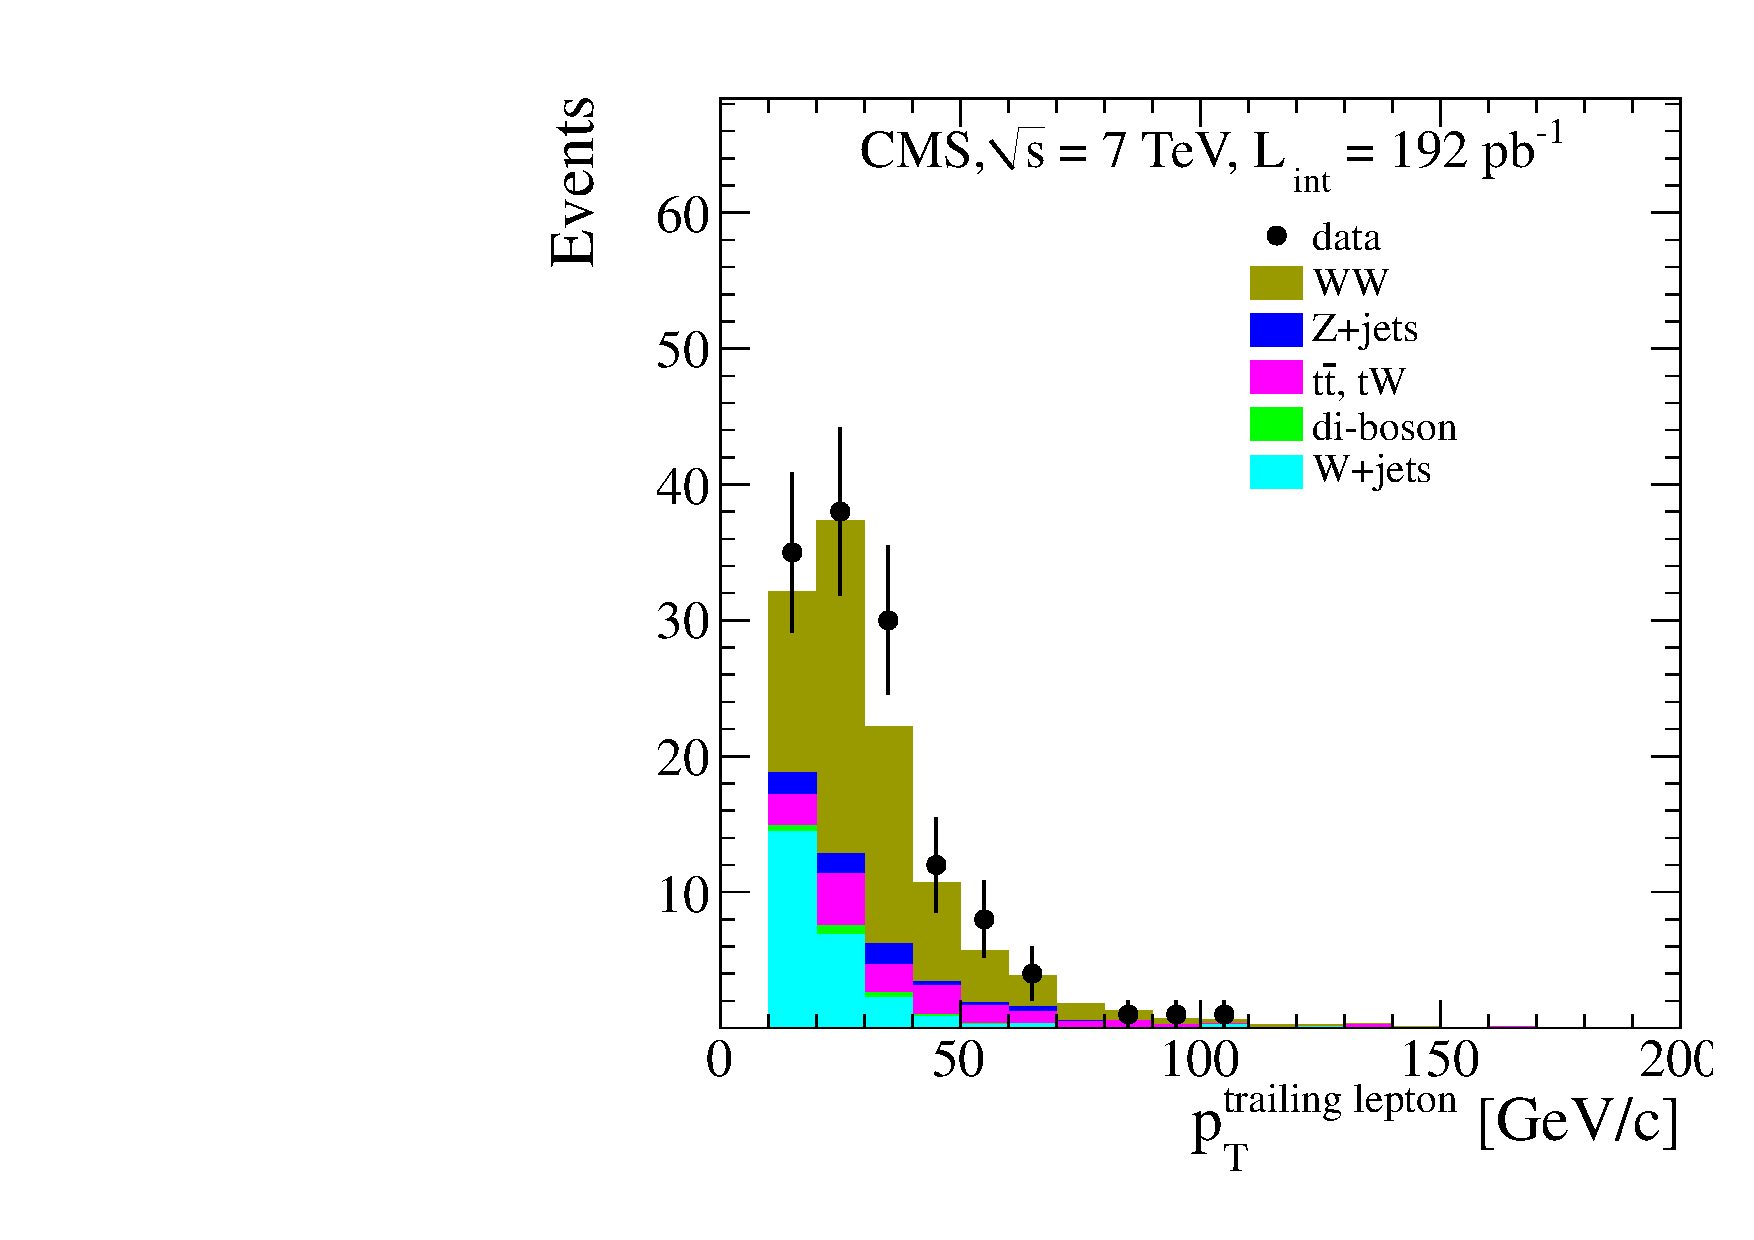
\includegraphics[width=.32\textwidth]{figures/ww_ptmin_0j.pdf}}
\subfigure[]{
\centering
\label{subfig:ww_ptmin_1j}
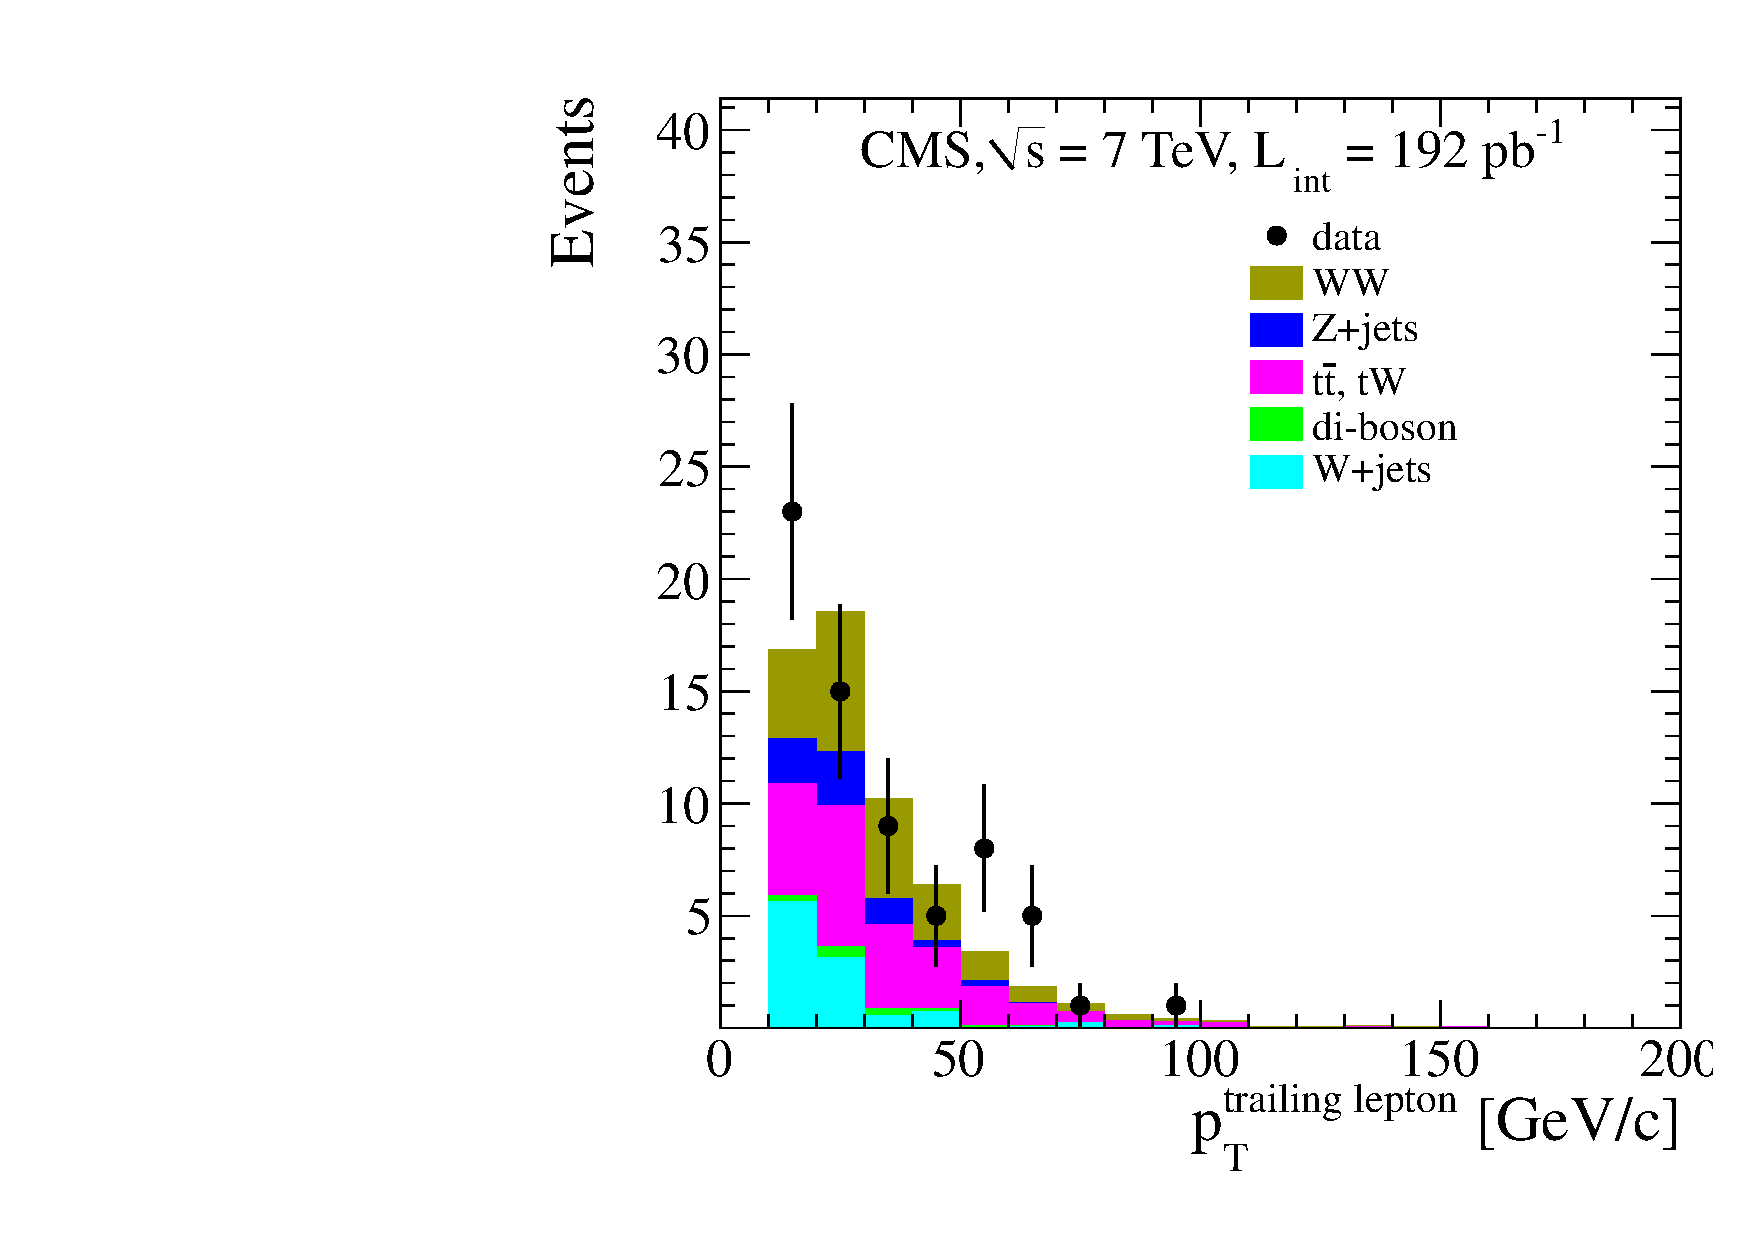
\includegraphics[width=.32\textwidth]{figures/ww_ptmin_1j.pdf}}
\subfigure[]{
\centering
\label{subfig:ww_ptmin_2j}
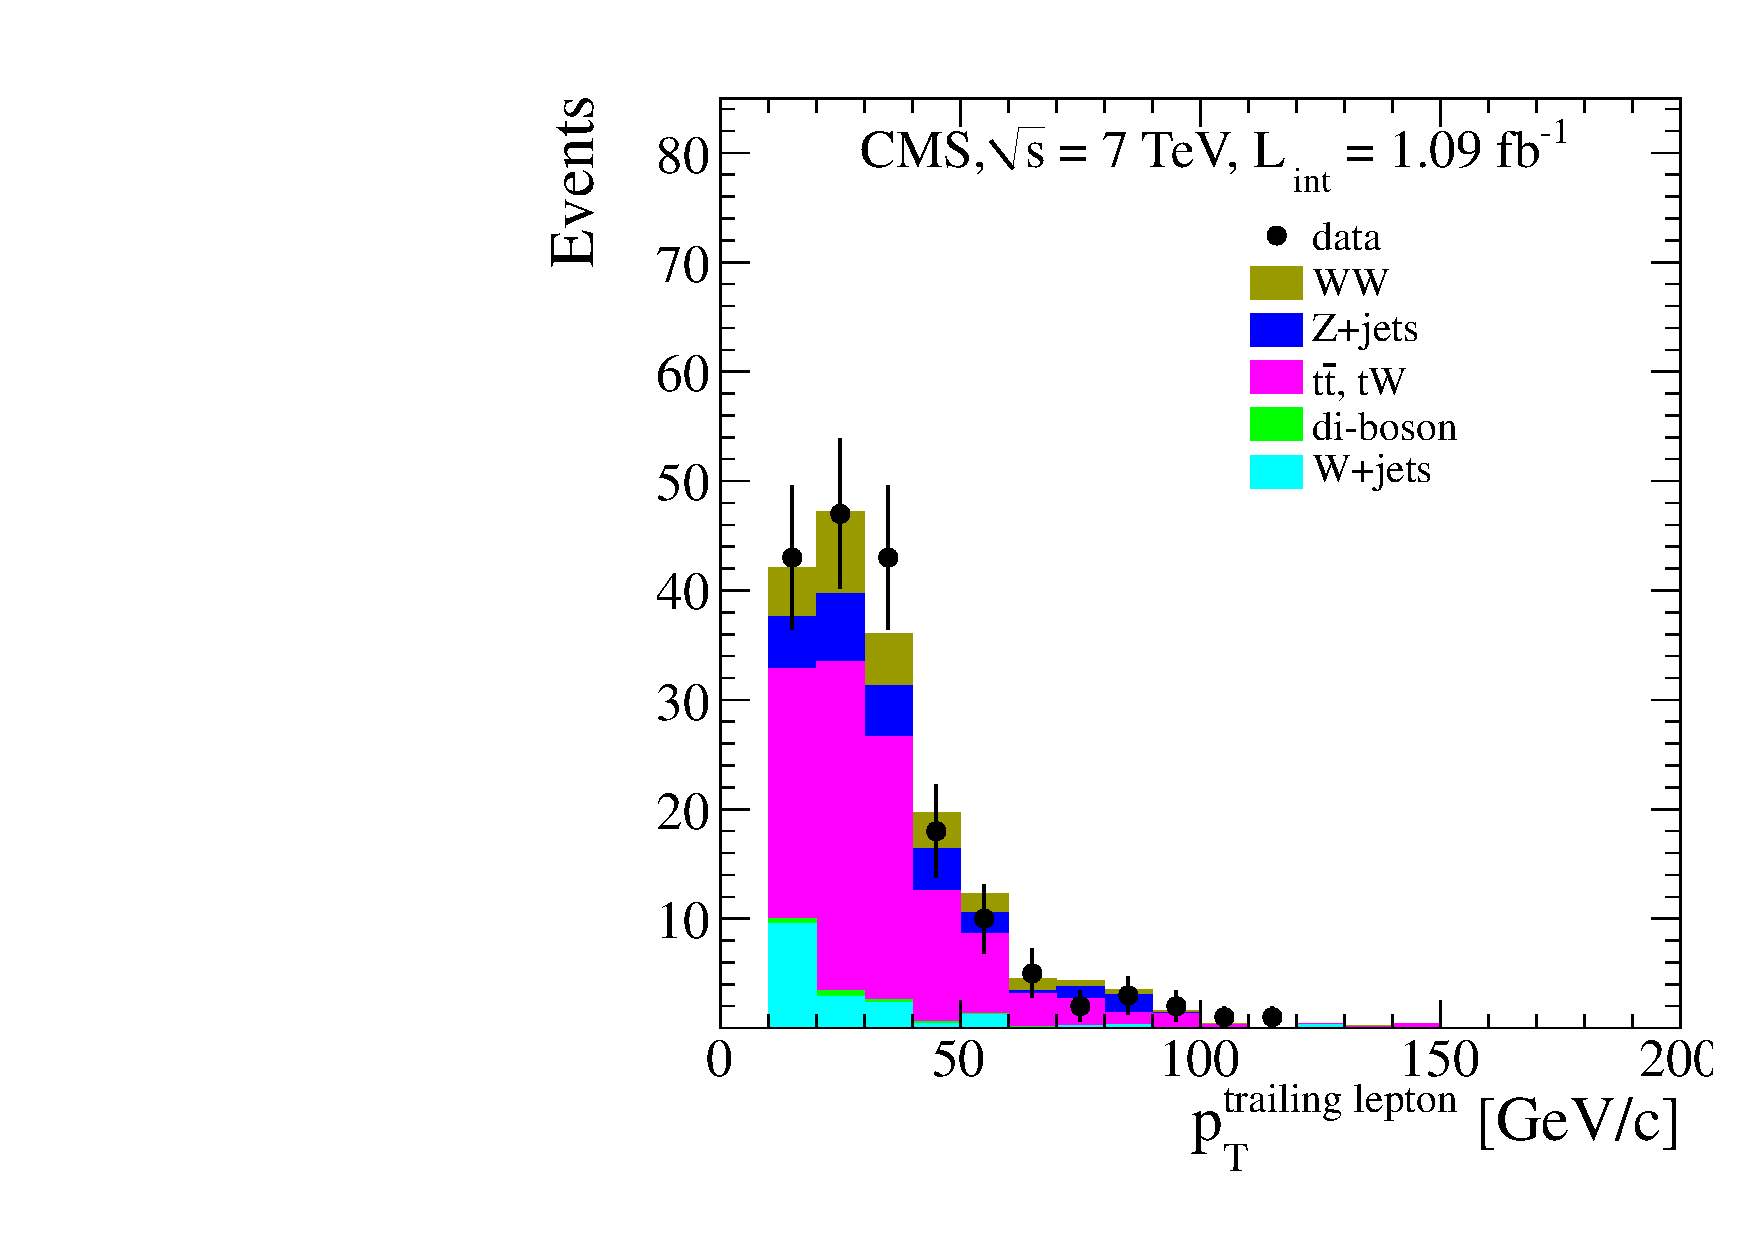
\includegraphics[width=.32\textwidth]{figures/ww_ptmin_2j.pdf}}\\
\caption{Trailing lepton $p_T$ distribution after WW selection for \intlumi of data in the 0-jet \subref{subfig:ww_ptmin_0j}, 
1-jet \subref{subfig:ww_ptmin_1j} and 2-jet \subref{subfig:ww_ptmin_2j} bin analyses. 
MC is scaled to data-driven estimates.}
\label{fig:ww_ptmin}
\end{figure}

\begin{figure}[!hbtp]
\centering
\subfigure[]{
\centering
\label{subfig:ww_ptmax_0j}
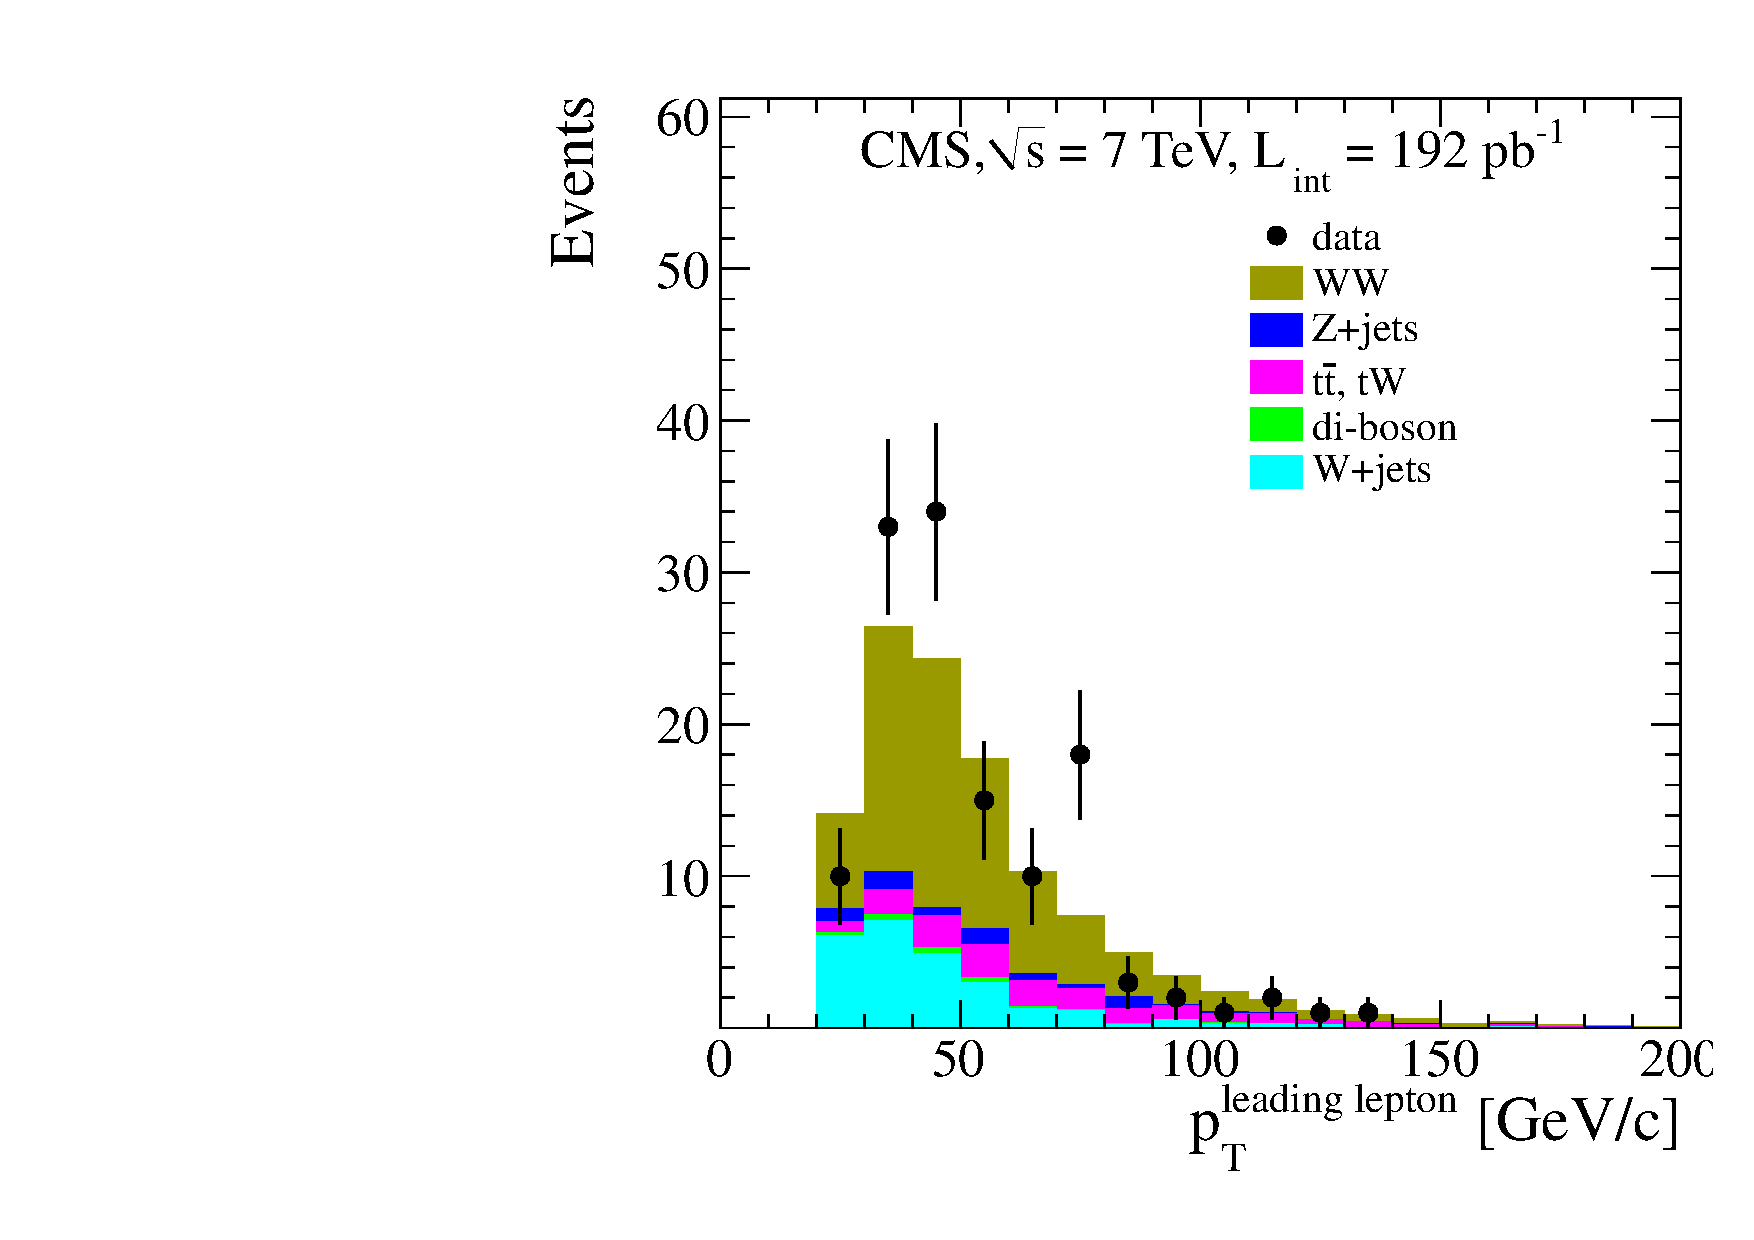
\includegraphics[width=.32\textwidth]{figures/ww_ptmax_0j.pdf}}
\subfigure[]{
\centering
\label{subfig:ww_ptmax_1j}
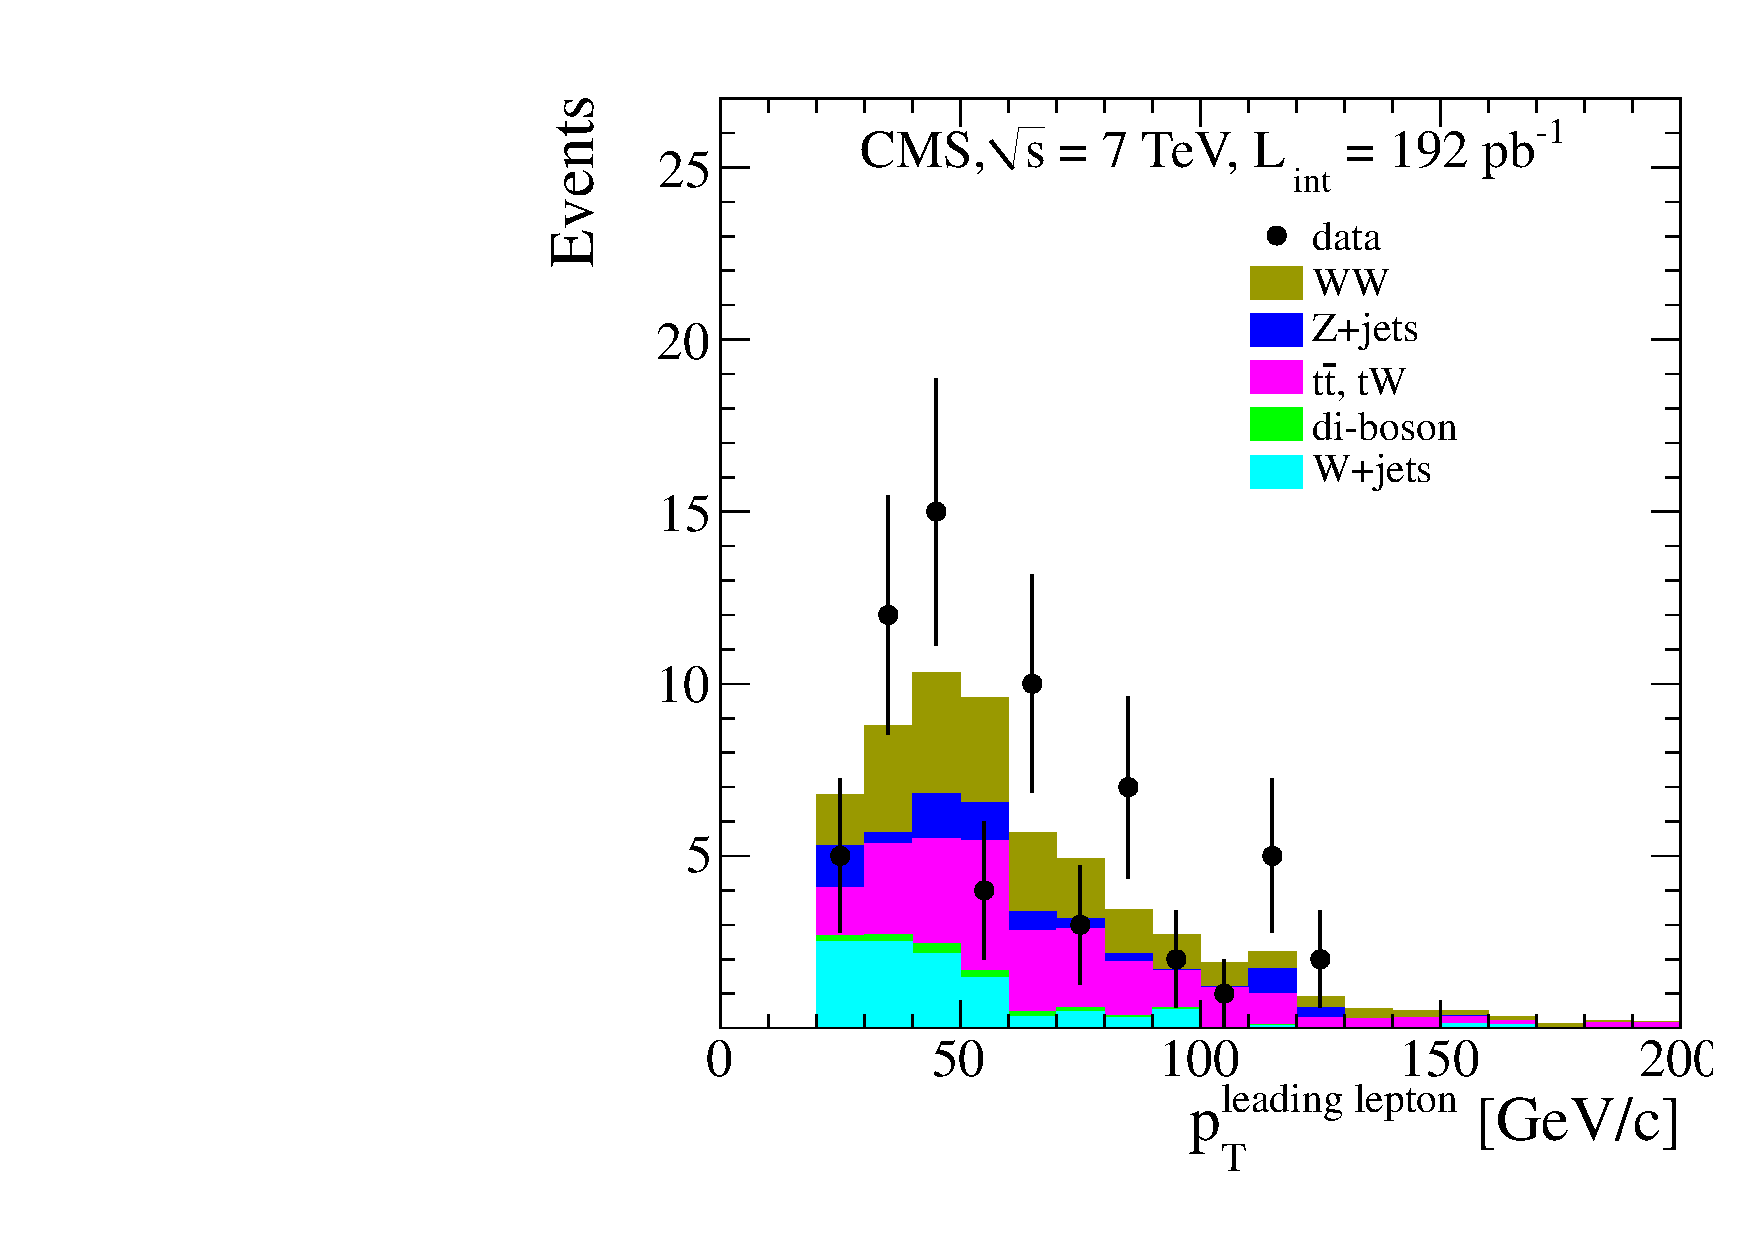
\includegraphics[width=.32\textwidth]{figures/ww_ptmax_1j.pdf}}
\subfigure[]{
\centering
\label{subfig:ww_ptmax_2j}
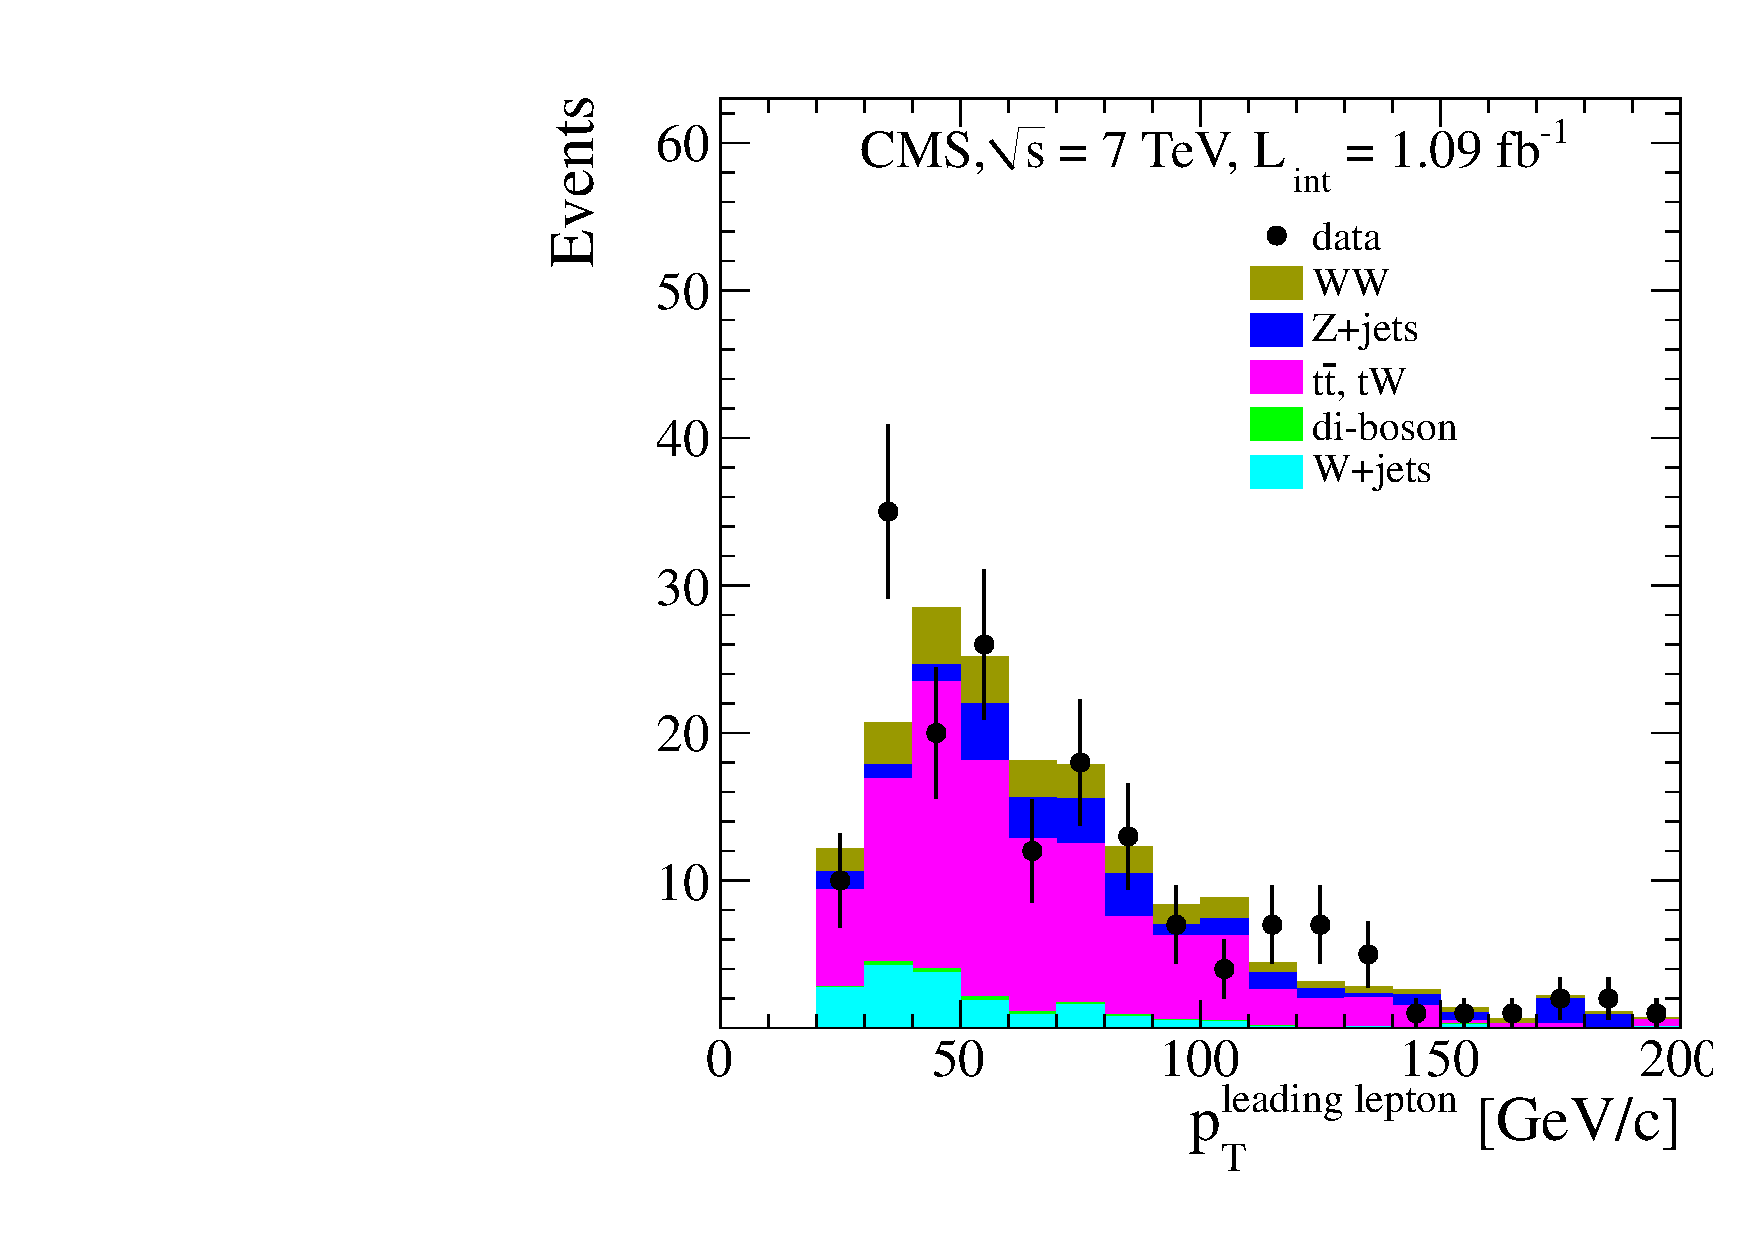
\includegraphics[width=.32\textwidth]{figures/ww_ptmax_2j.pdf}}\\
\caption{Leading lepton $p_T$ distribution after WW selection for \intlumi of data in the 0-jet \subref{subfig:ww_ptmax_0j}, 
1-jet \subref{subfig:ww_ptmax_1j} and 2-jet \subref{subfig:ww_ptmax_2j} bin analyses. 
MC is scaled to data-driven estimates.}
\label{fig:ww_ptmax}
\end{figure}

\begin{figure}[!hbtp]
\centering
\subfigure[]{
\centering
\label{subfig:ww_pmet_0j}
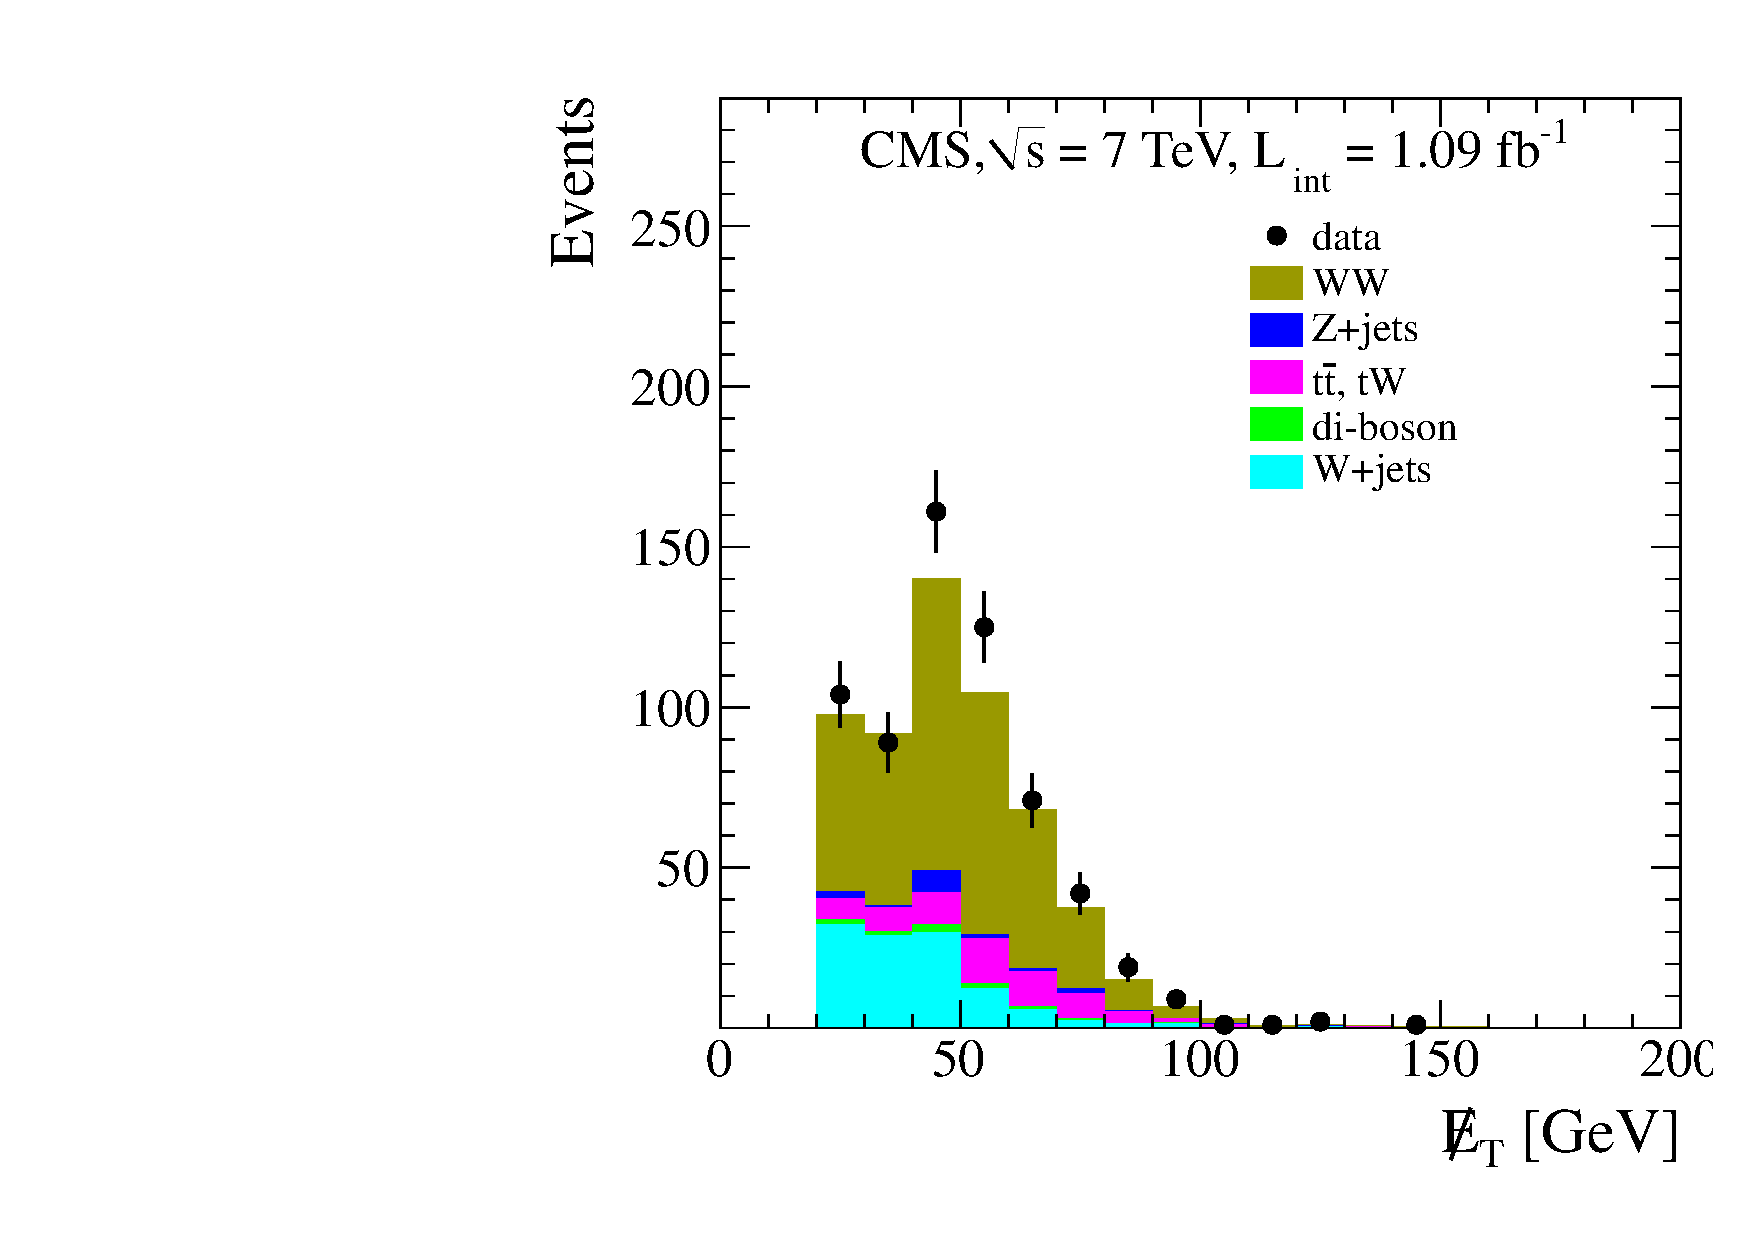
\includegraphics[width=.32\textwidth]{figures/ww_pmet_0j.pdf}}
\subfigure[]{
\centering
\label{subfig:ww_pmet_1j}
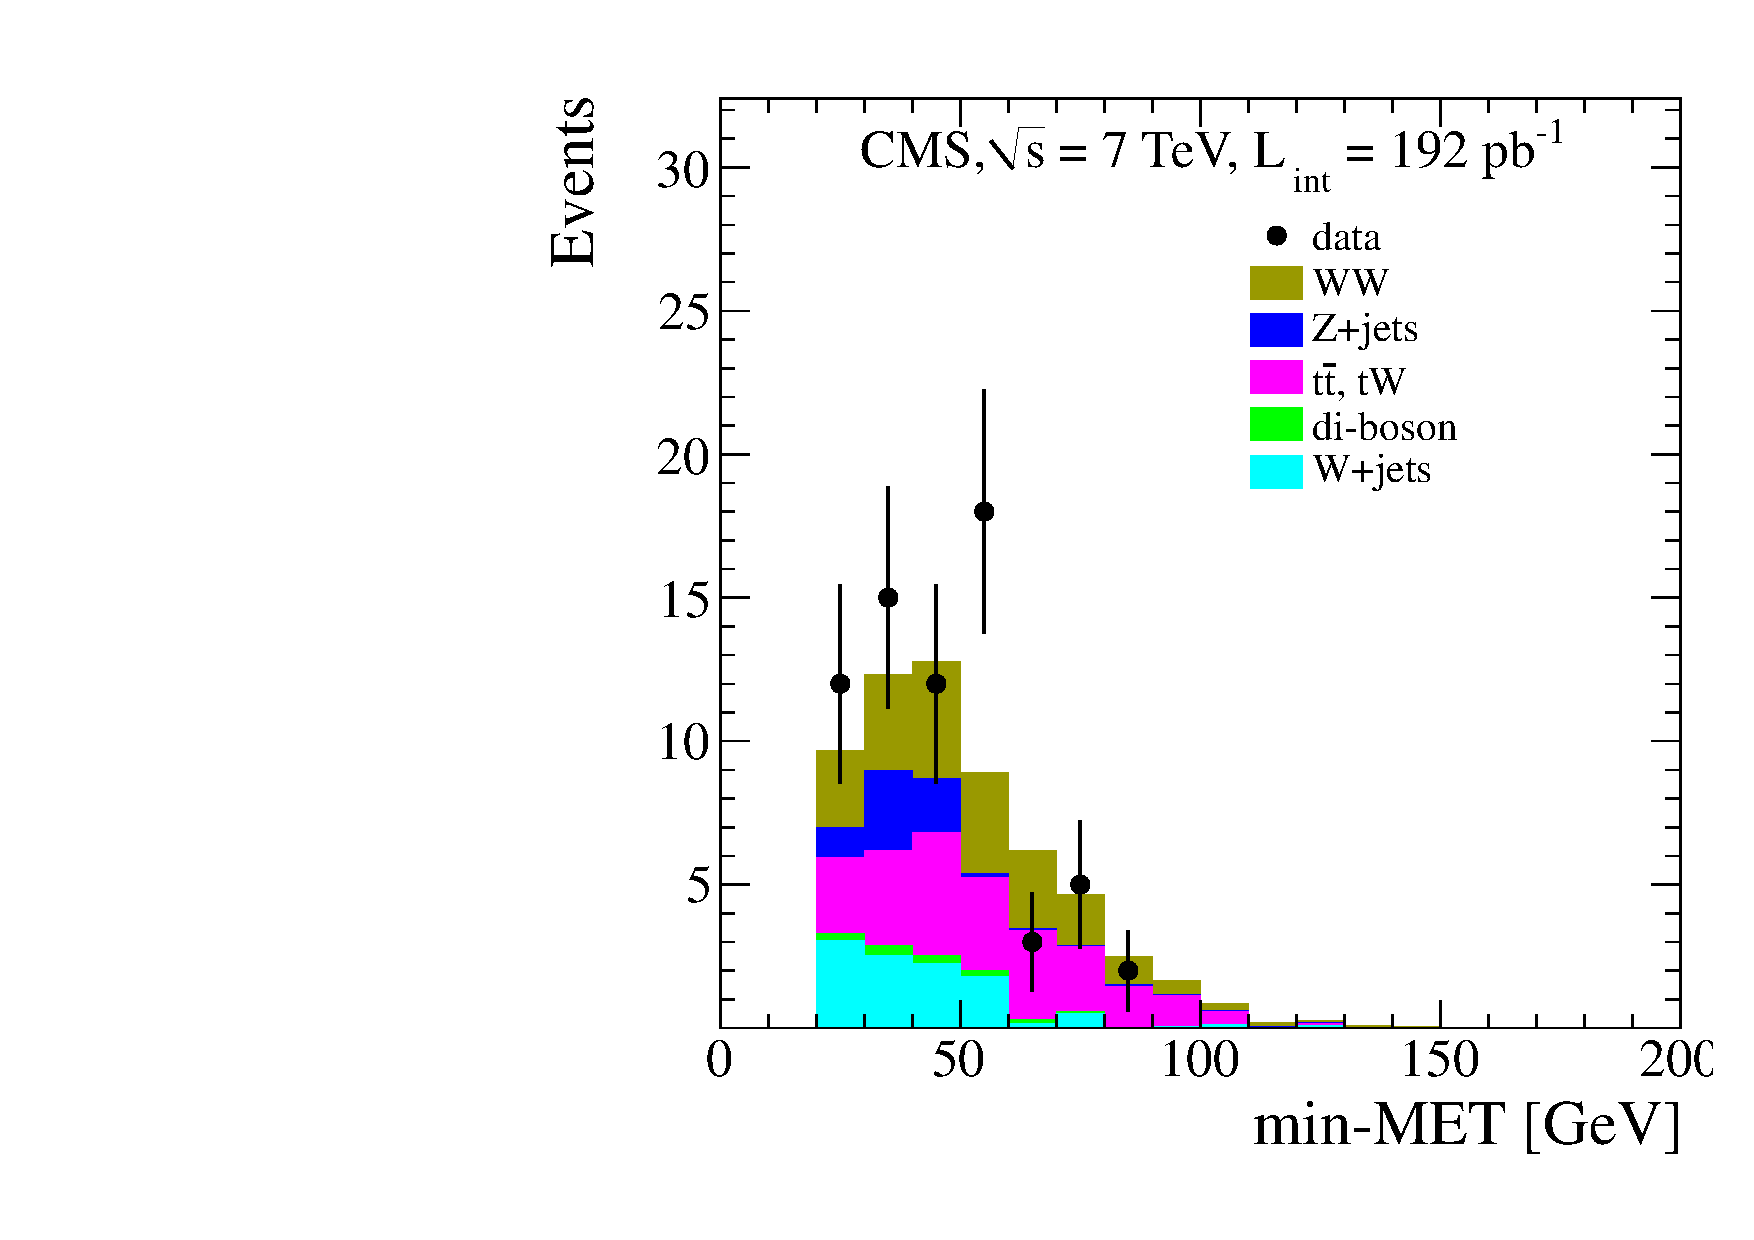
\includegraphics[width=.32\textwidth]{figures/ww_pmet_1j.pdf}}
\subfigure[]{
\centering
\label{subfig:ww_pmet_2j}
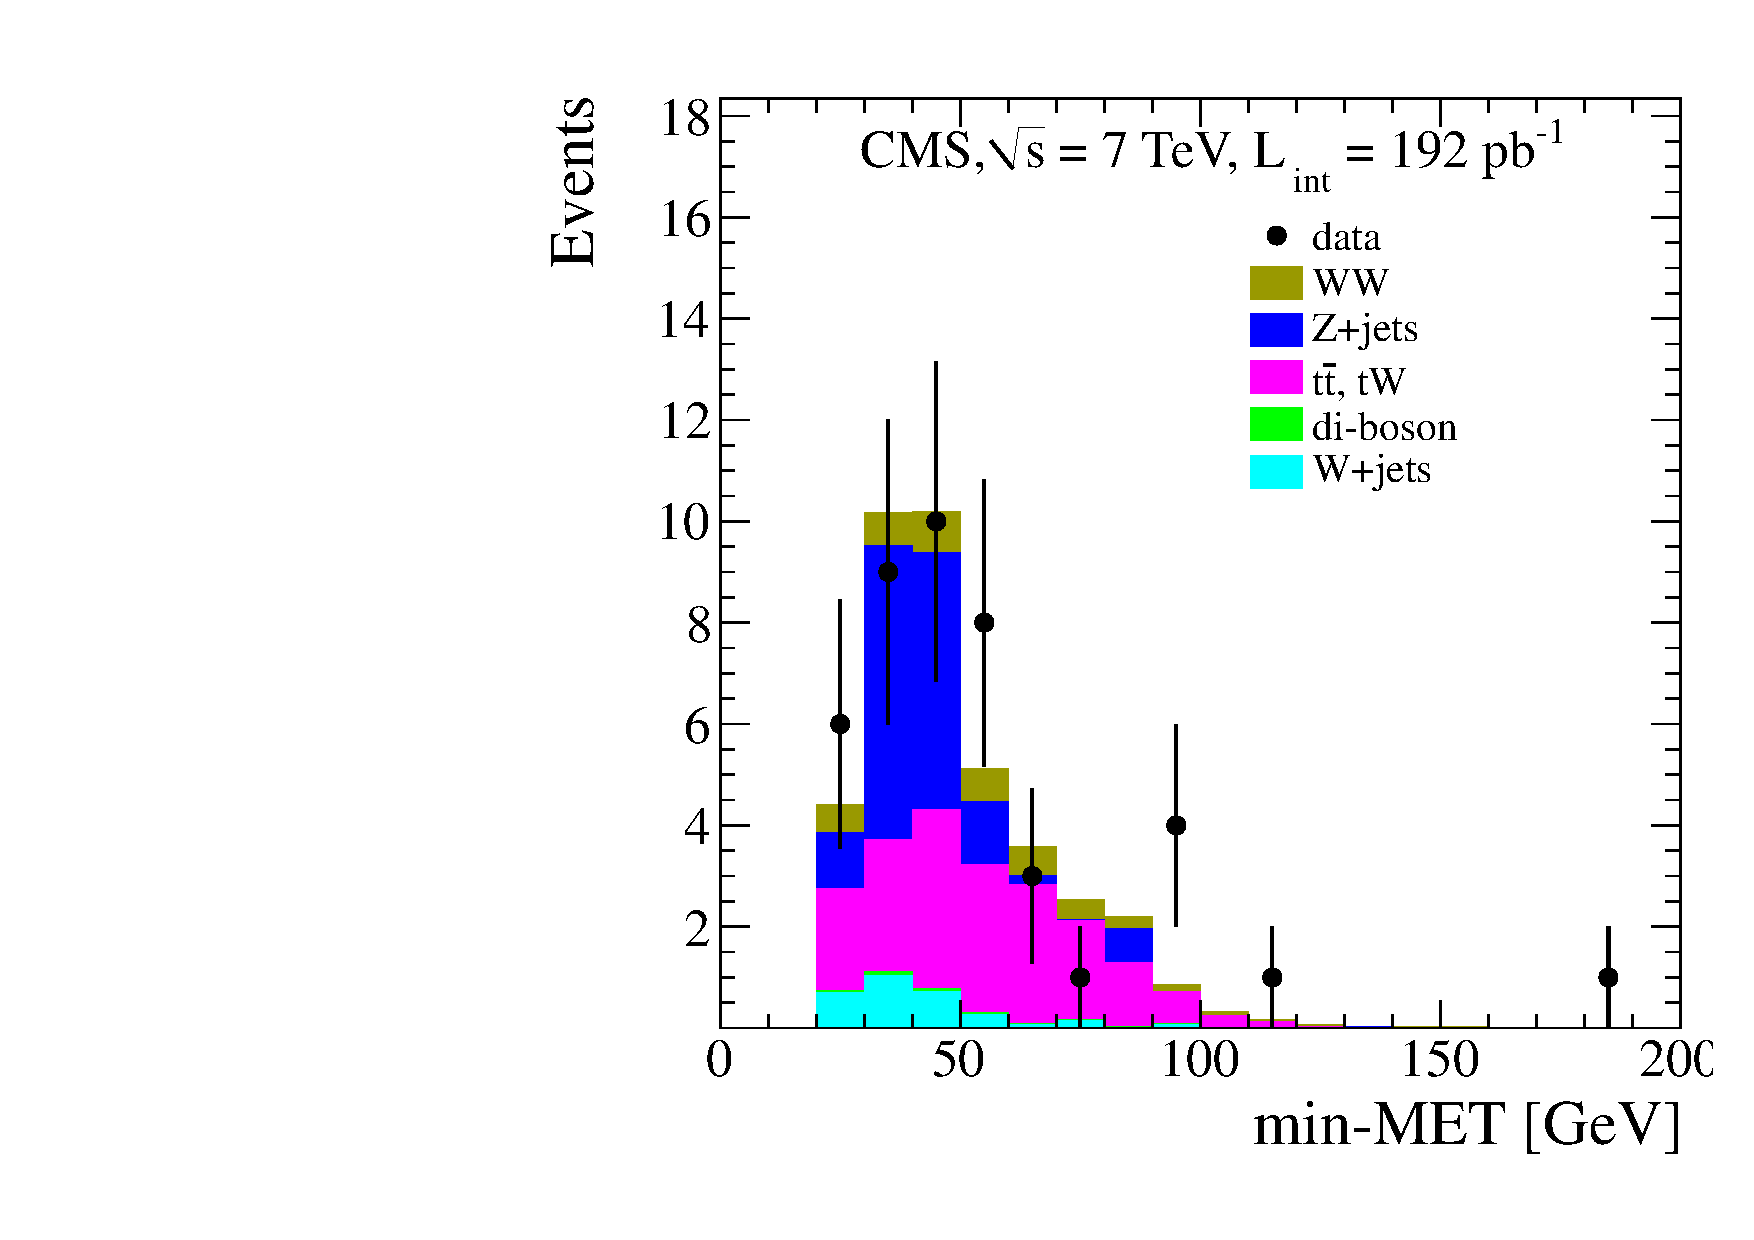
\includegraphics[width=.32\textwidth]{figures/ww_pmet_2j.pdf}}\\
\caption{$min(\text{proj}_\text{trk-MET}, \text{proj}_\text{PFMET})$ distribution after WW selection for \intlumi of data in the 0-jet \subref{subfig:ww_pmet_0j}, 
1-jet \subref{subfig:ww_pmet_1j} and 2-jet \subref{subfig:ww_pmet_2j} bin analyses. 
MC is scaled to data-driven estimates.}
\label{fig:ww_pmet}
\end{figure}

\begin{figure}[!hbtp]
\centering
\subfigure[]{
\centering
\label{subfig:ww_mt_0j}
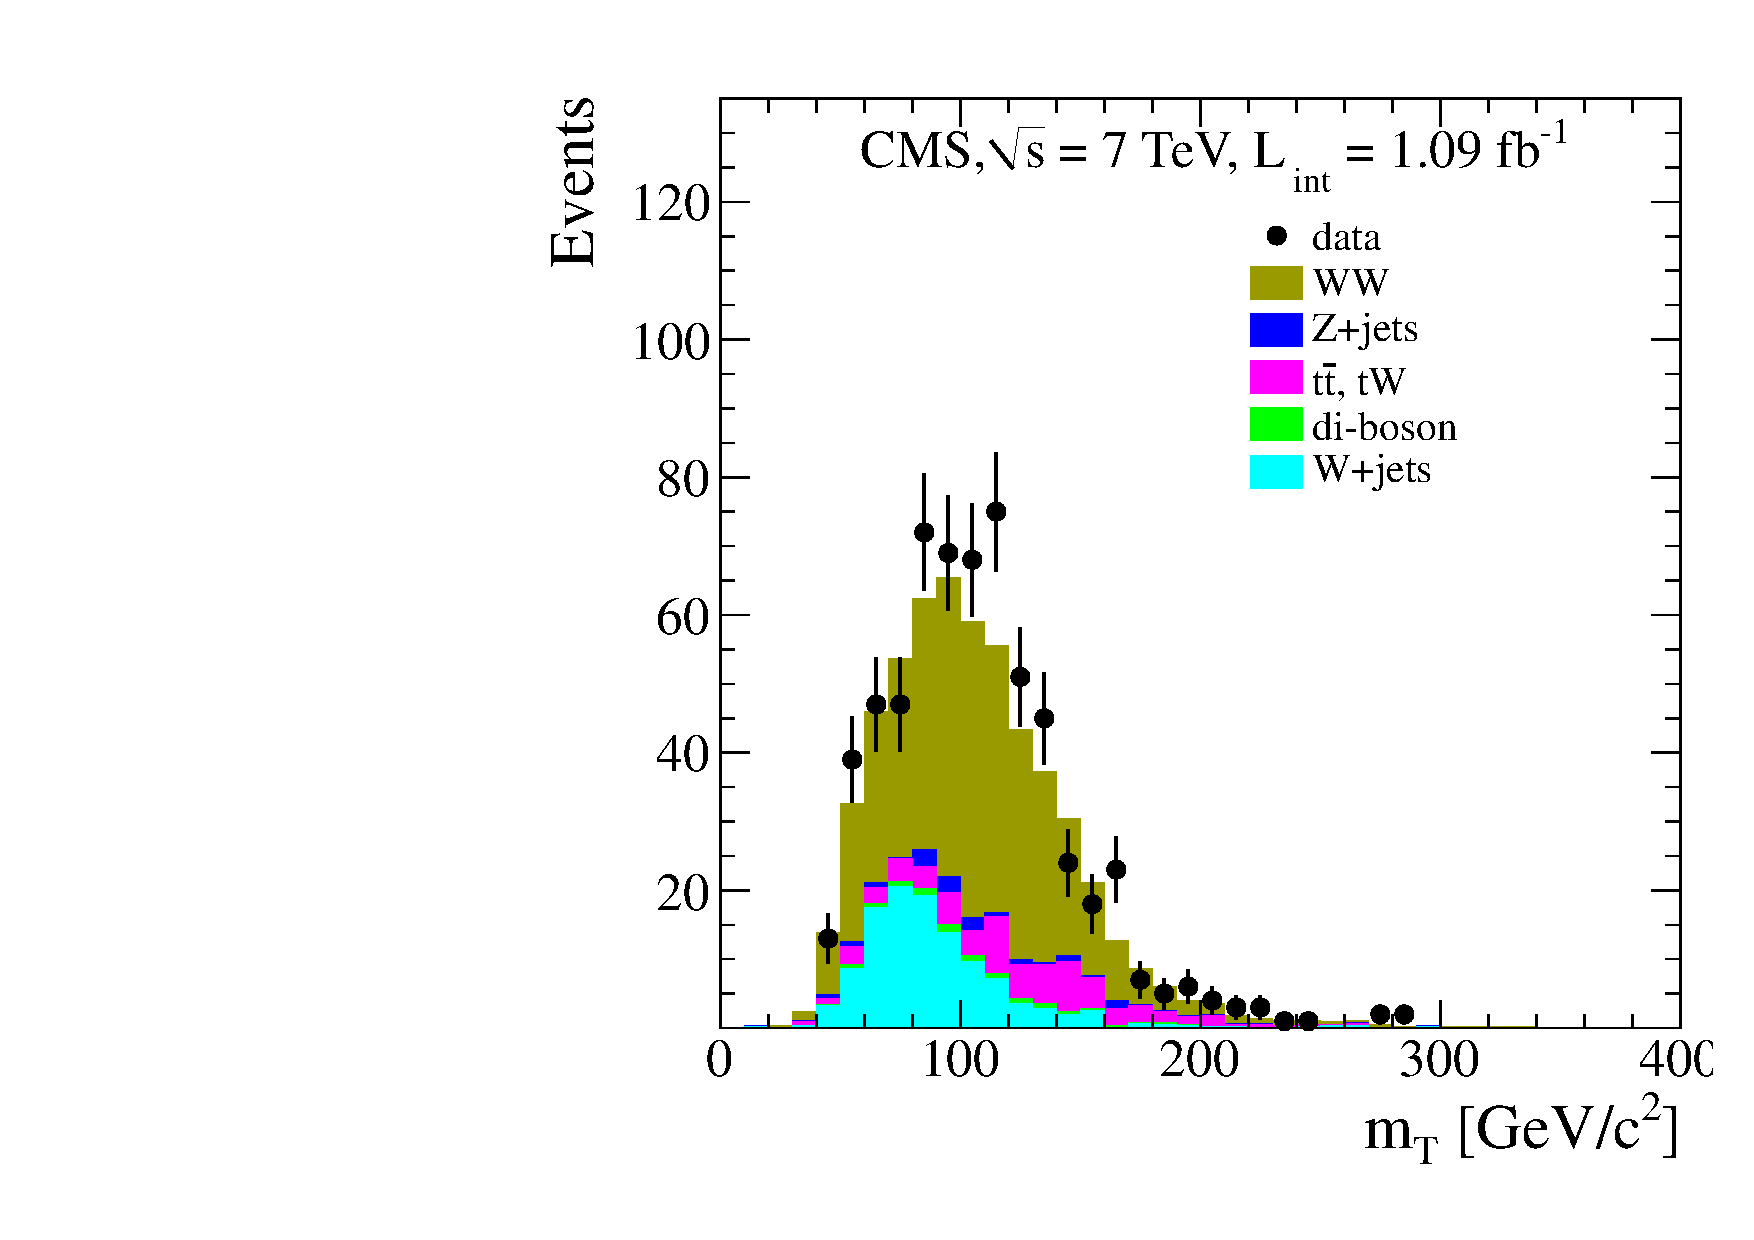
\includegraphics[width=.32\textwidth]{figures/ww_mt_0j.pdf}}
\subfigure[]{
\centering
\label{subfig:ww_mt_1j}
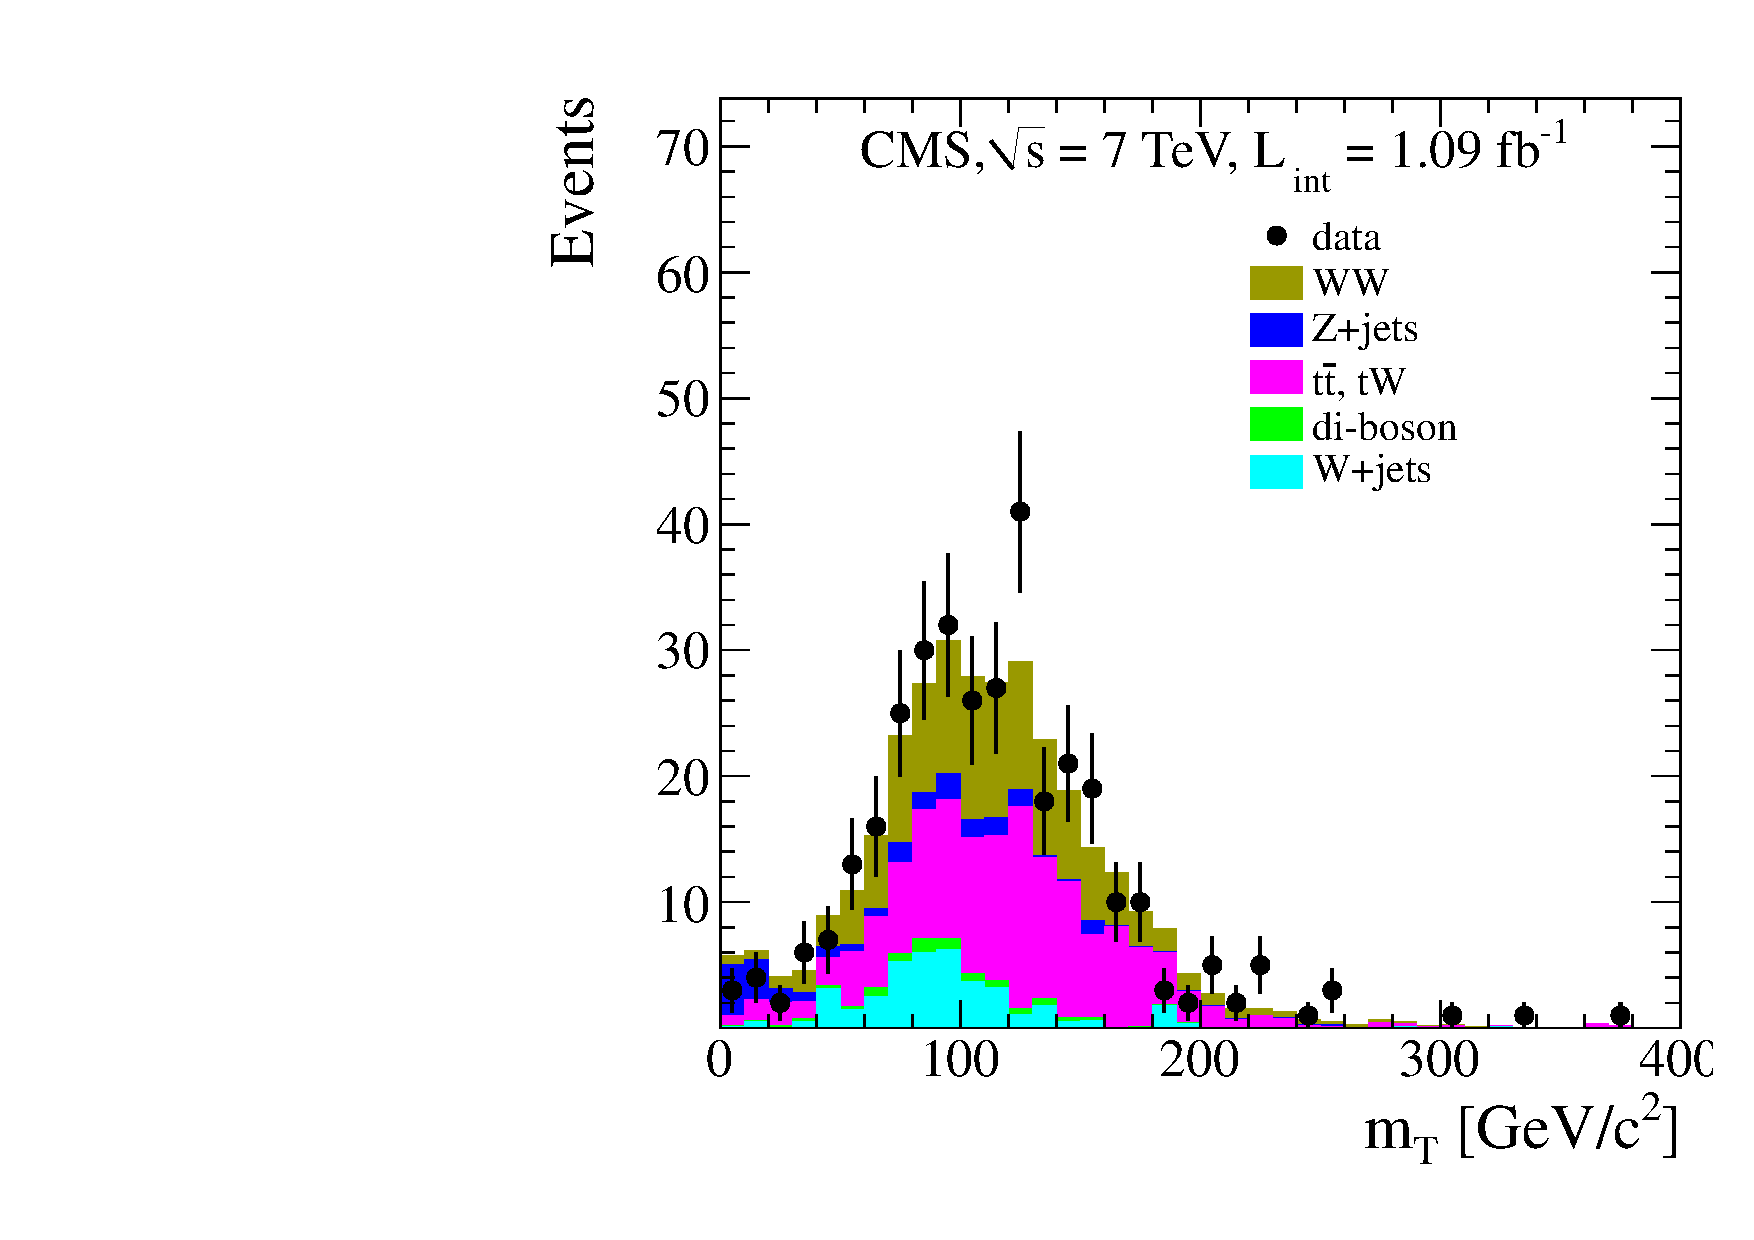
\includegraphics[width=.32\textwidth]{figures/ww_mt_1j.pdf}}
\subfigure[]{
\centering
\label{subfig:ww_mt_2j}
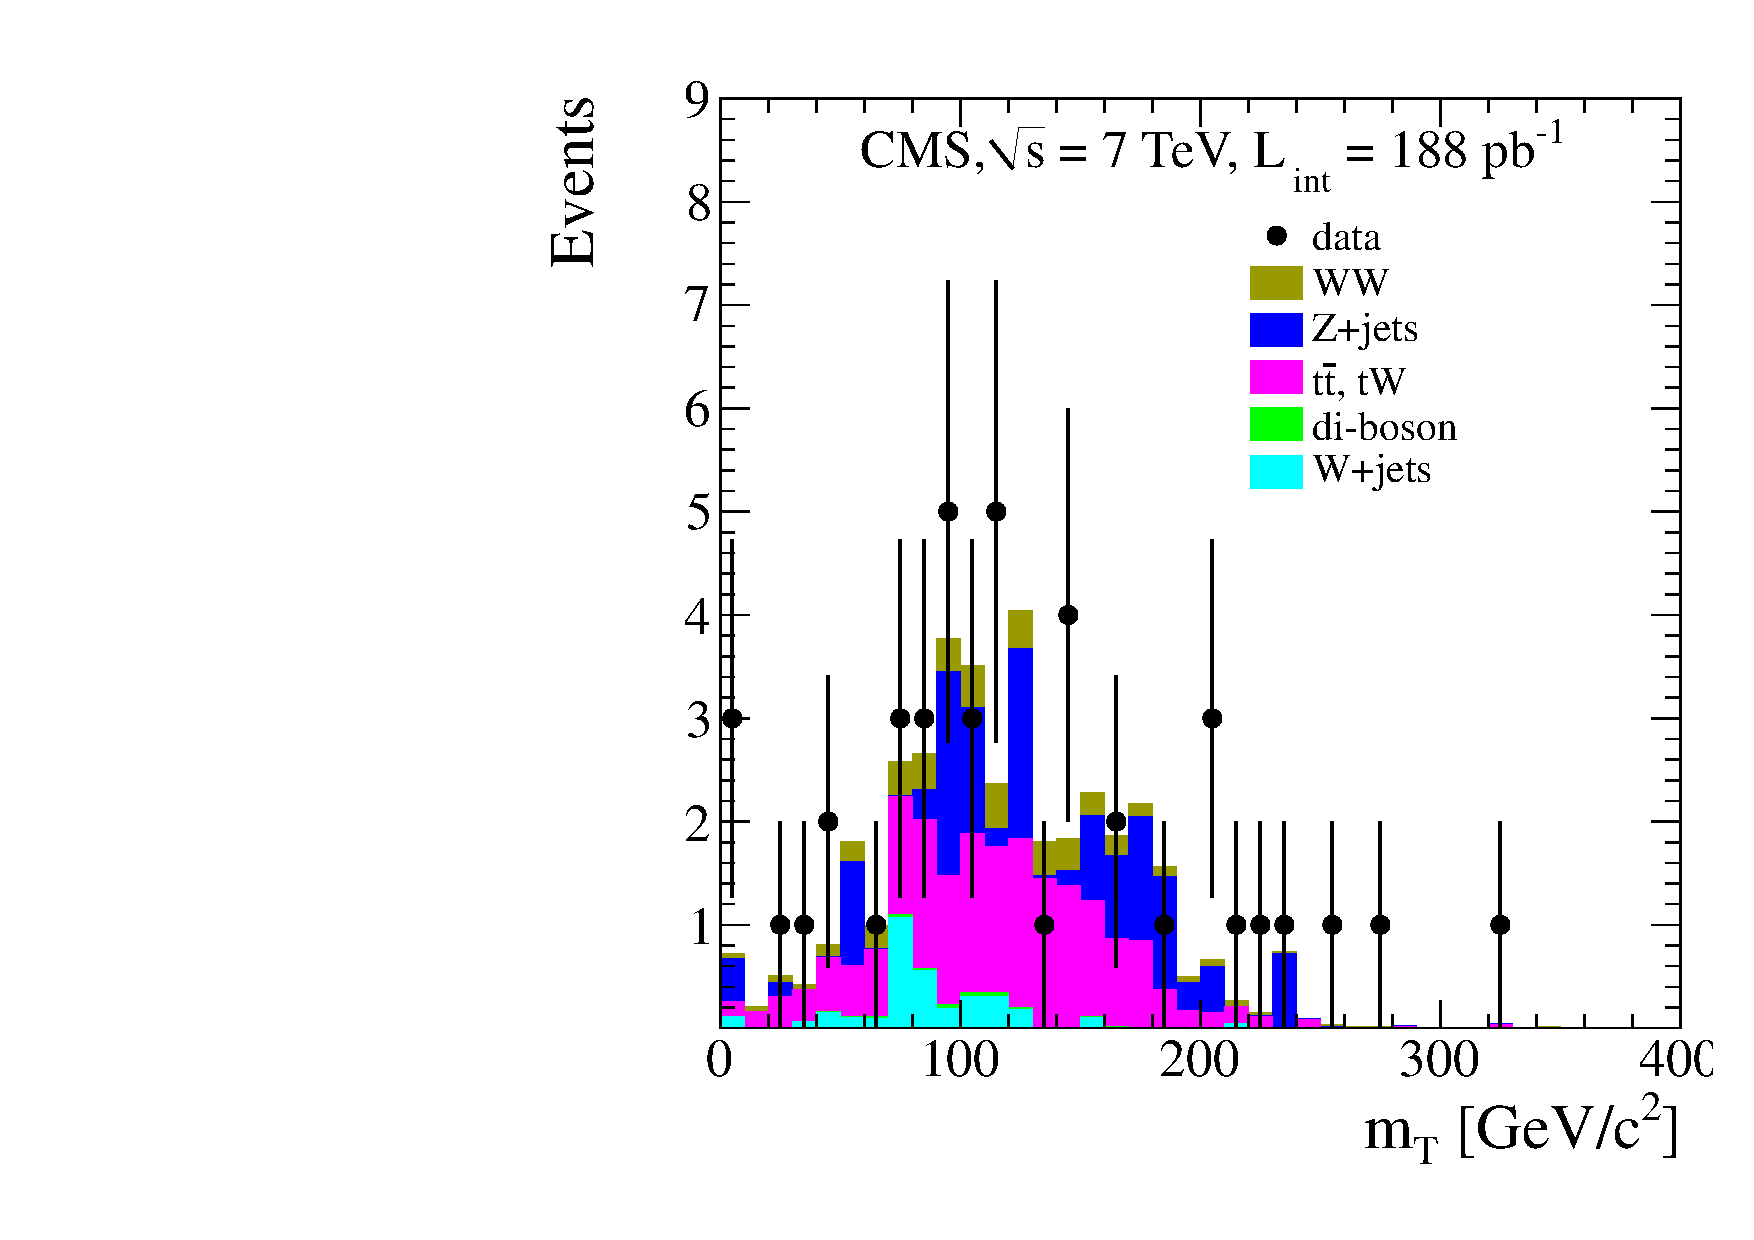
\includegraphics[width=.32\textwidth]{figures/ww_mt_2j.pdf}}\\
\caption{Transverse mass distribution after WW selection for \intlumi of data in the 0-jet \subref{subfig:ww_mt_0j}, 
1-jet \subref{subfig:ww_mt_1j} and 2-jet \subref{subfig:ww_mt_2j} bin analyses. 
MC is scaled to data-driven estimates.}
\label{fig:ww_mt}
\end{figure}

\begin{figure}[!hbtp]
\centering
\subfigure[]{
\centering
\label{subfig:ww_dilmass_0j}
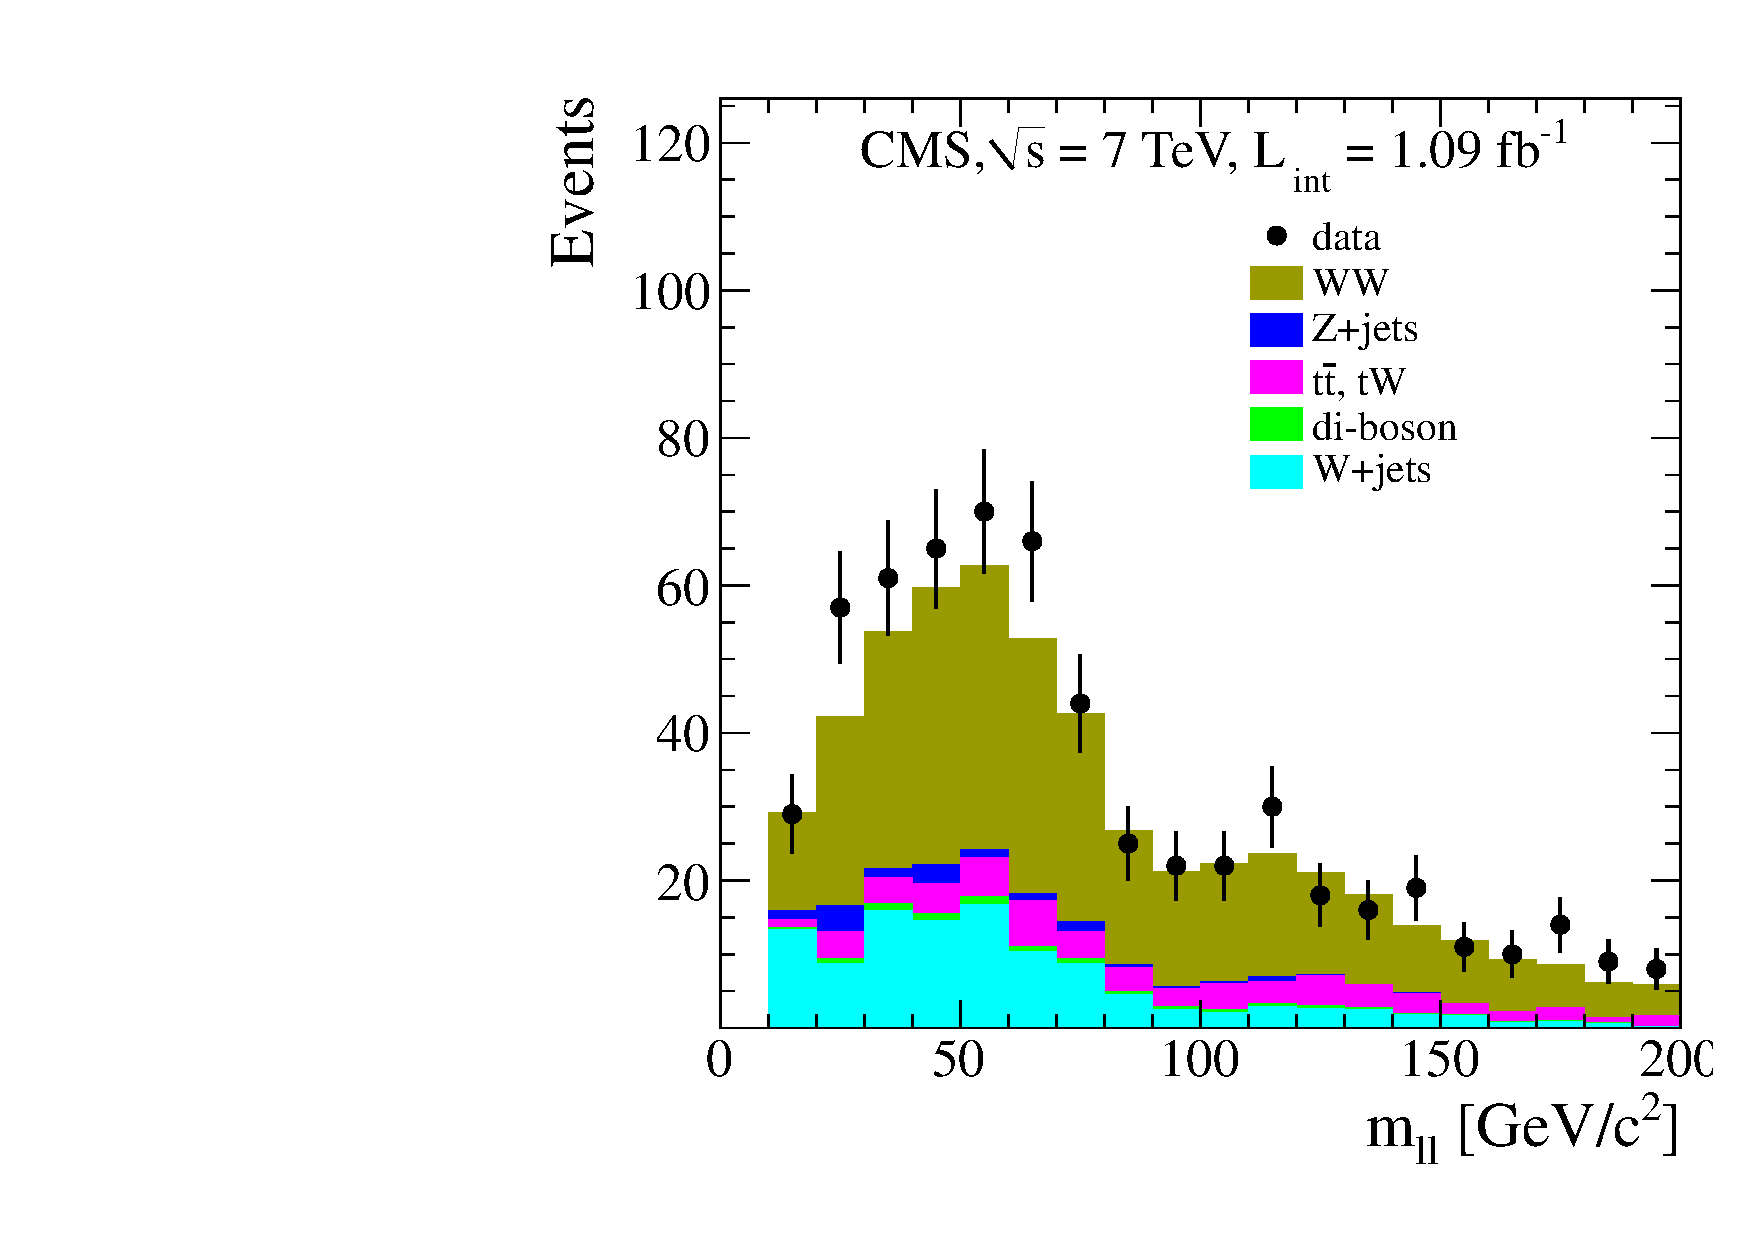
\includegraphics[width=.32\textwidth]{figures/ww_dilmass_0j.pdf}}
\subfigure[]{
\centering
\label{subfig:ww_dilmass_1j}
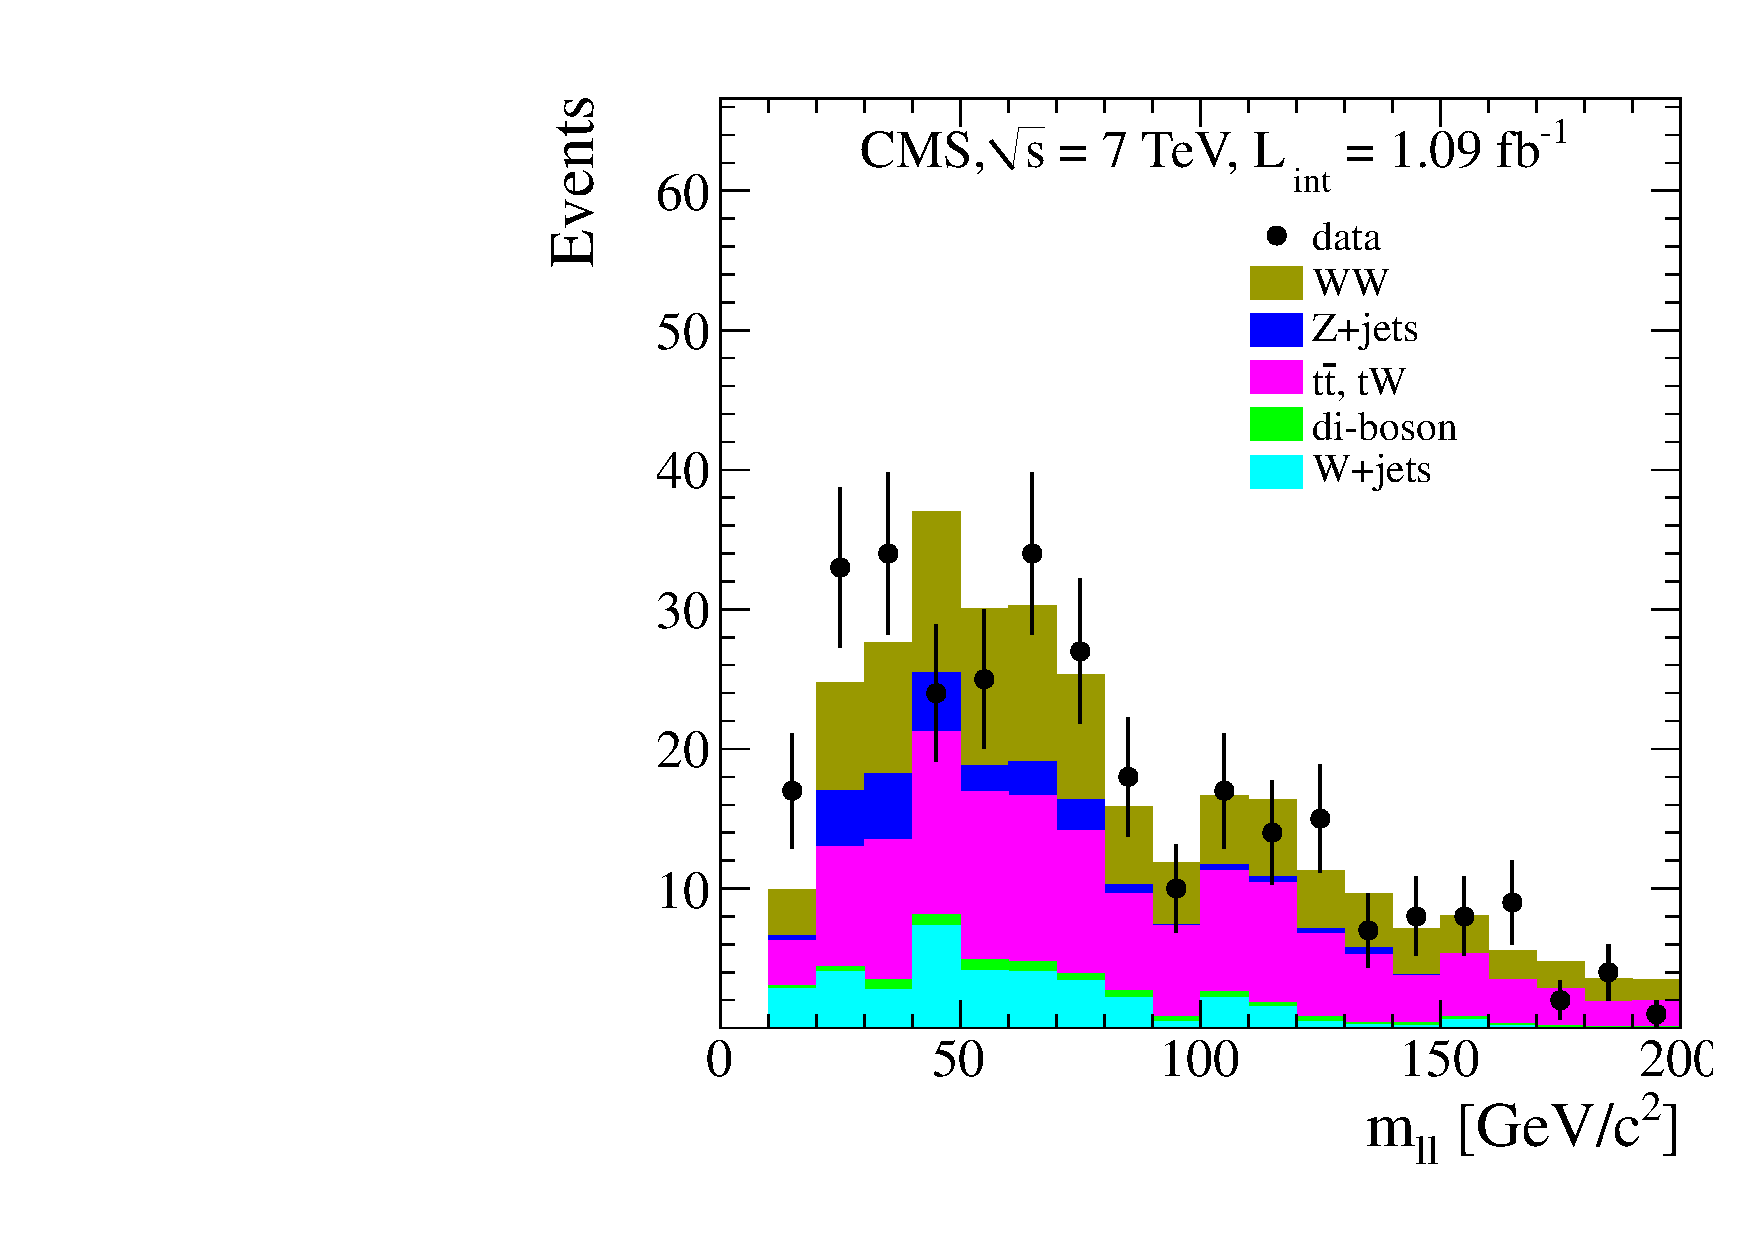
\includegraphics[width=.32\textwidth]{figures/ww_dilmass_1j.pdf}}
\subfigure[]{
\centering
\label{subfig:ww_dilmass_2j}
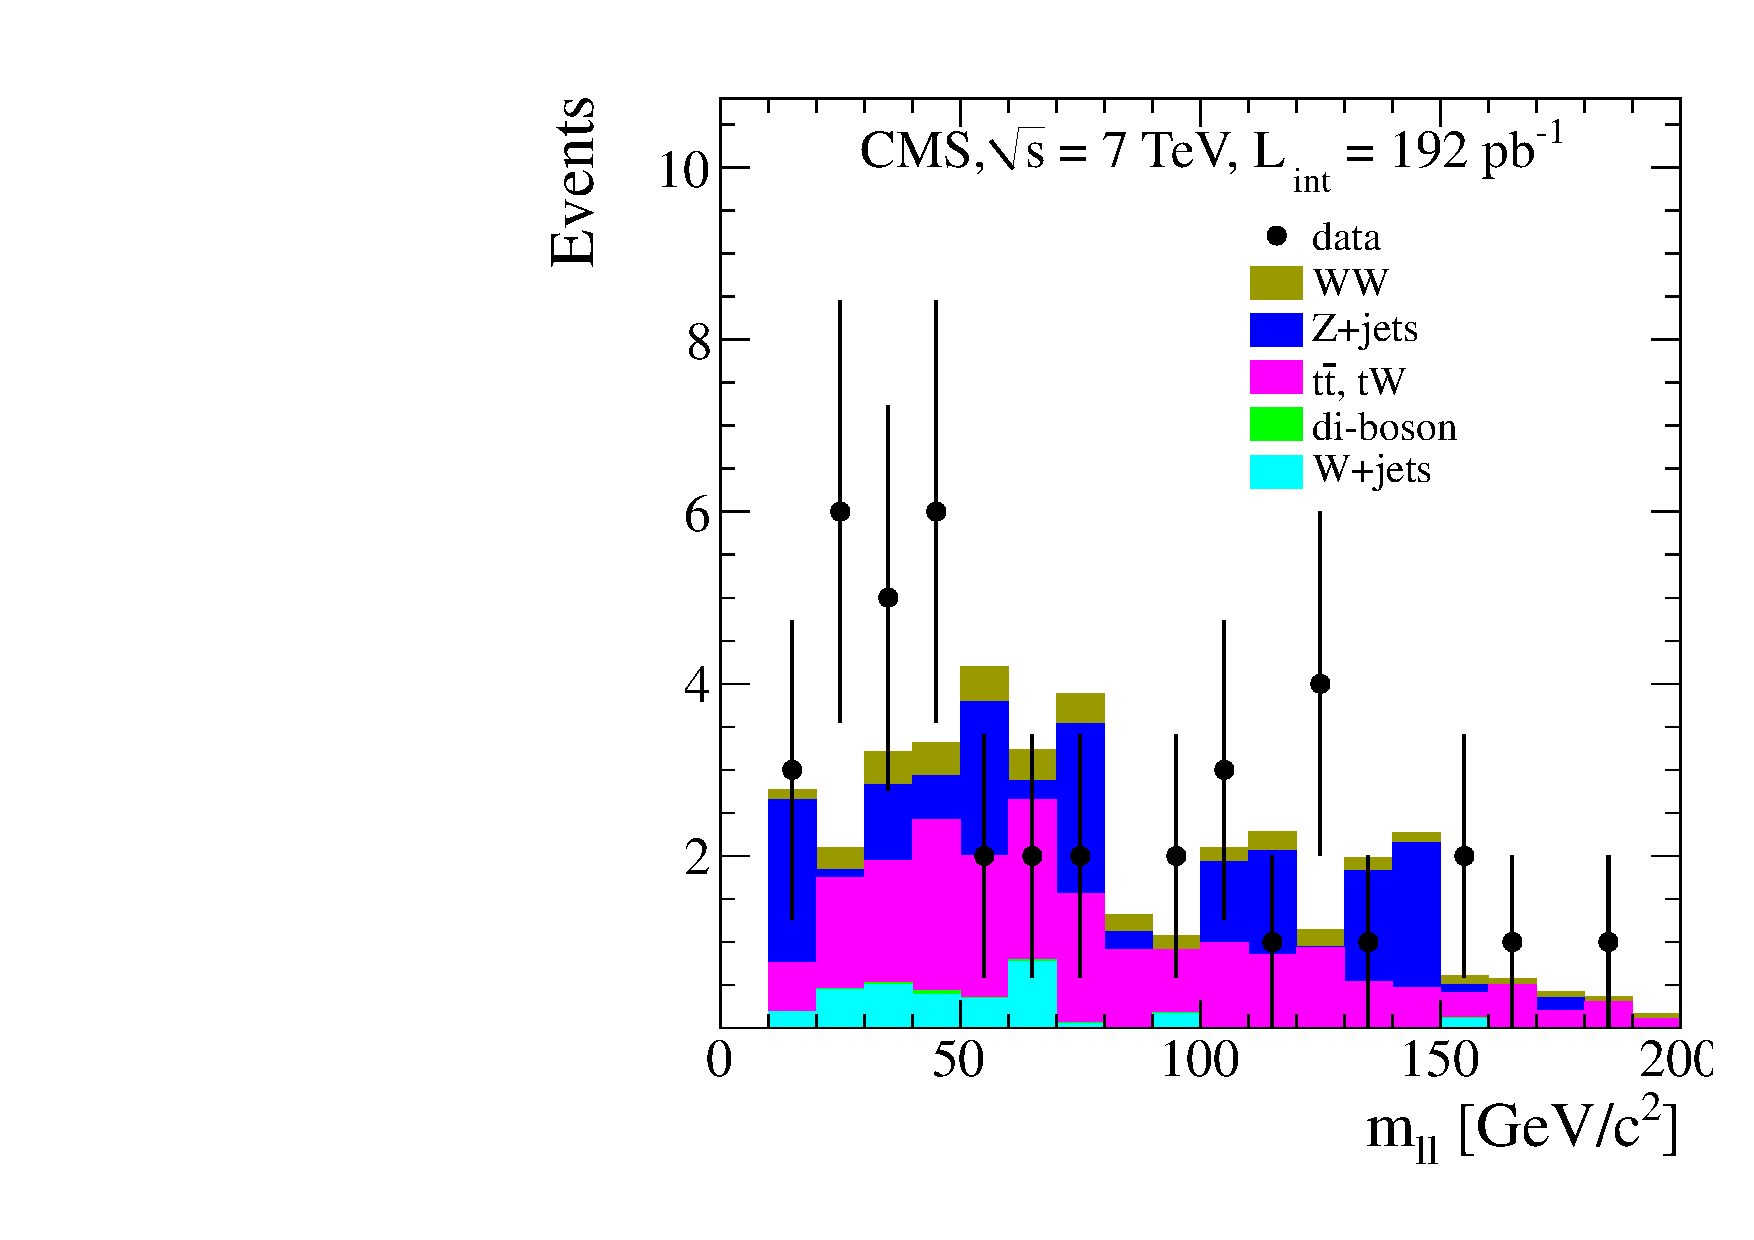
\includegraphics[width=.32\textwidth]{figures/ww_dilmass_2j.pdf}}\\
\caption{Invariant dilepton mass distribution after WW selection for \intlumi of data in the 0-jet \subref{subfig:ww_dilmass_0j}, 
1-jet \subref{subfig:ww_dilmass_1j} and 2-jet \subref{subfig:ww_dilmass_2j} bin analyses. 
MC is scaled to data-driven estimates.}
\label{fig:ww_dilmass}
\end{figure}

\begin{figure}[!hbtp]
\centering
\subfigure[]{
\centering
\label{subfig:ww_deltaphi_0j}
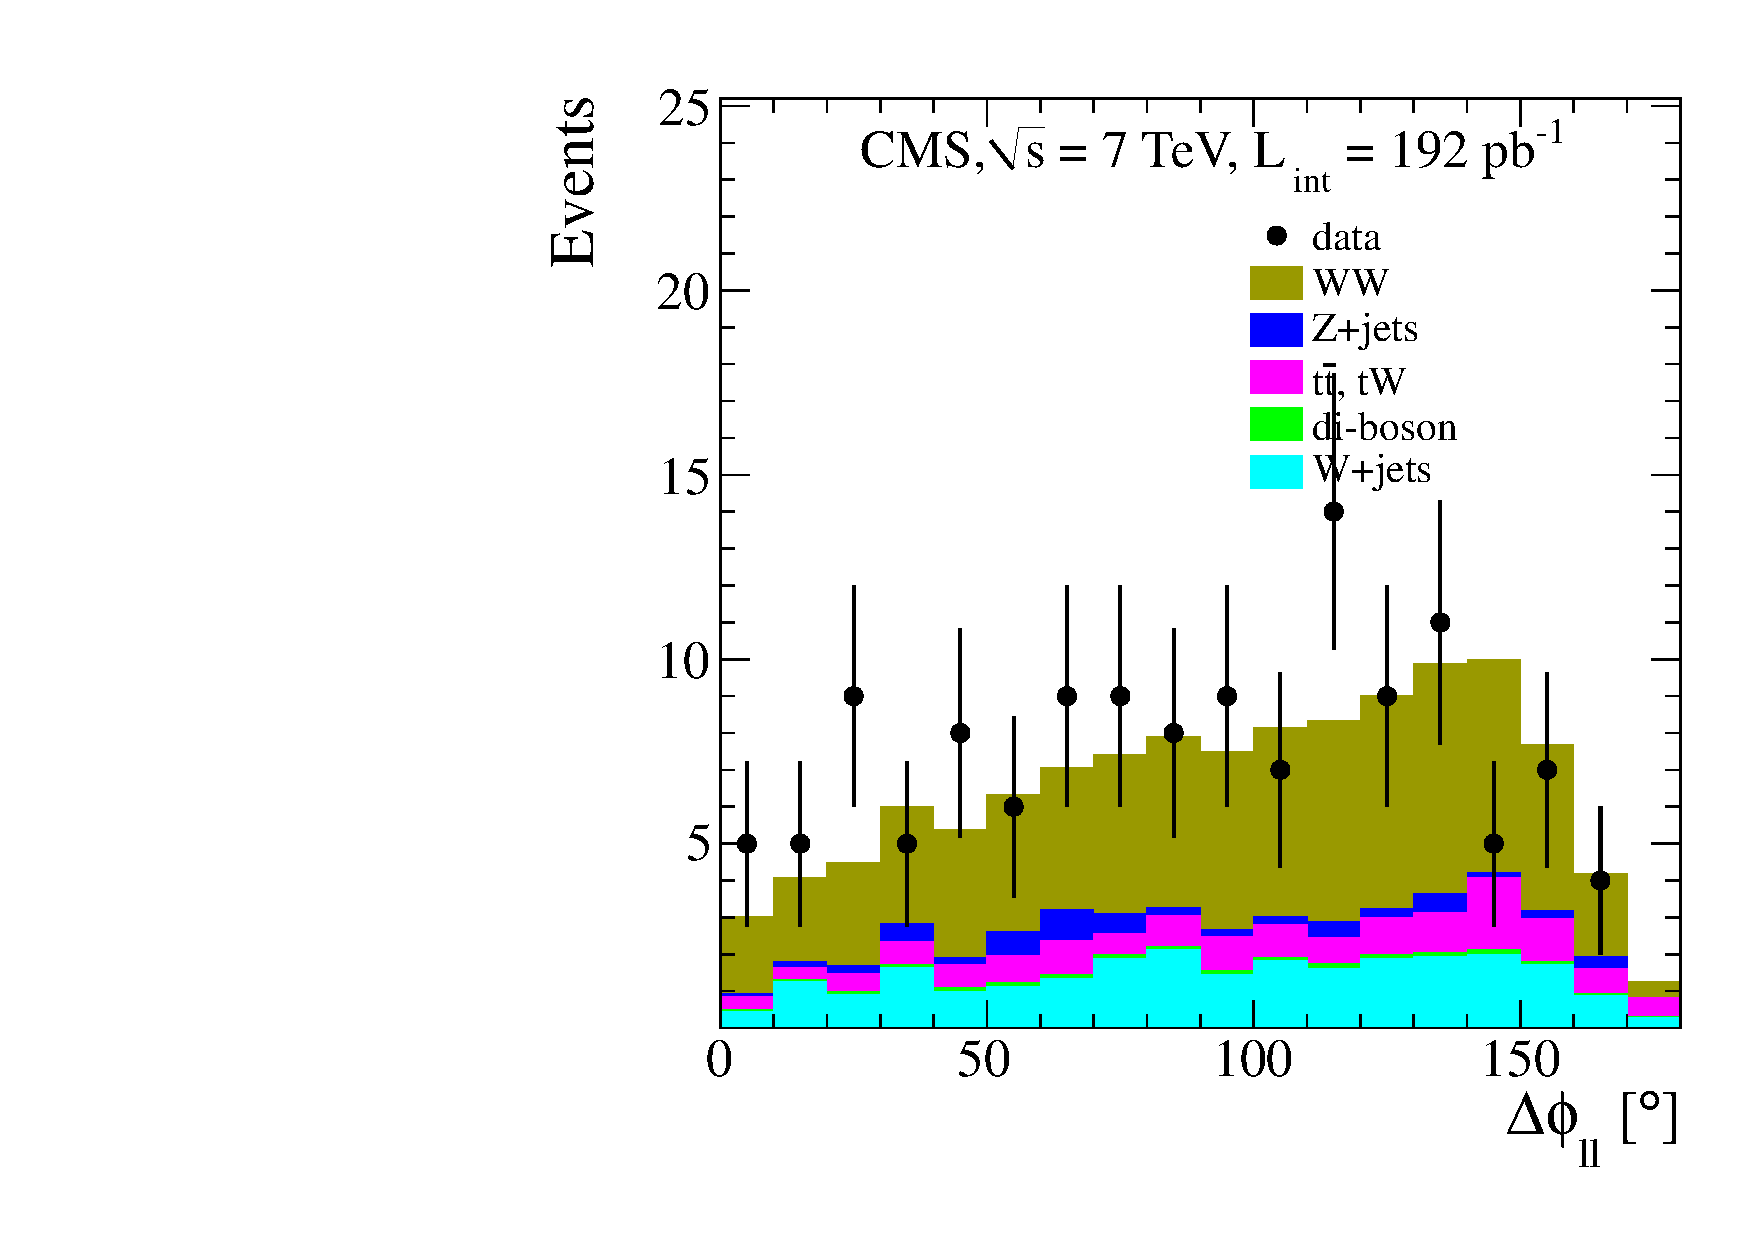
\includegraphics[width=.32\textwidth]{figures/ww_deltaphi_0j.pdf}}
\subfigure[]{
\centering
\label{subfig:ww_deltaphi_1j}
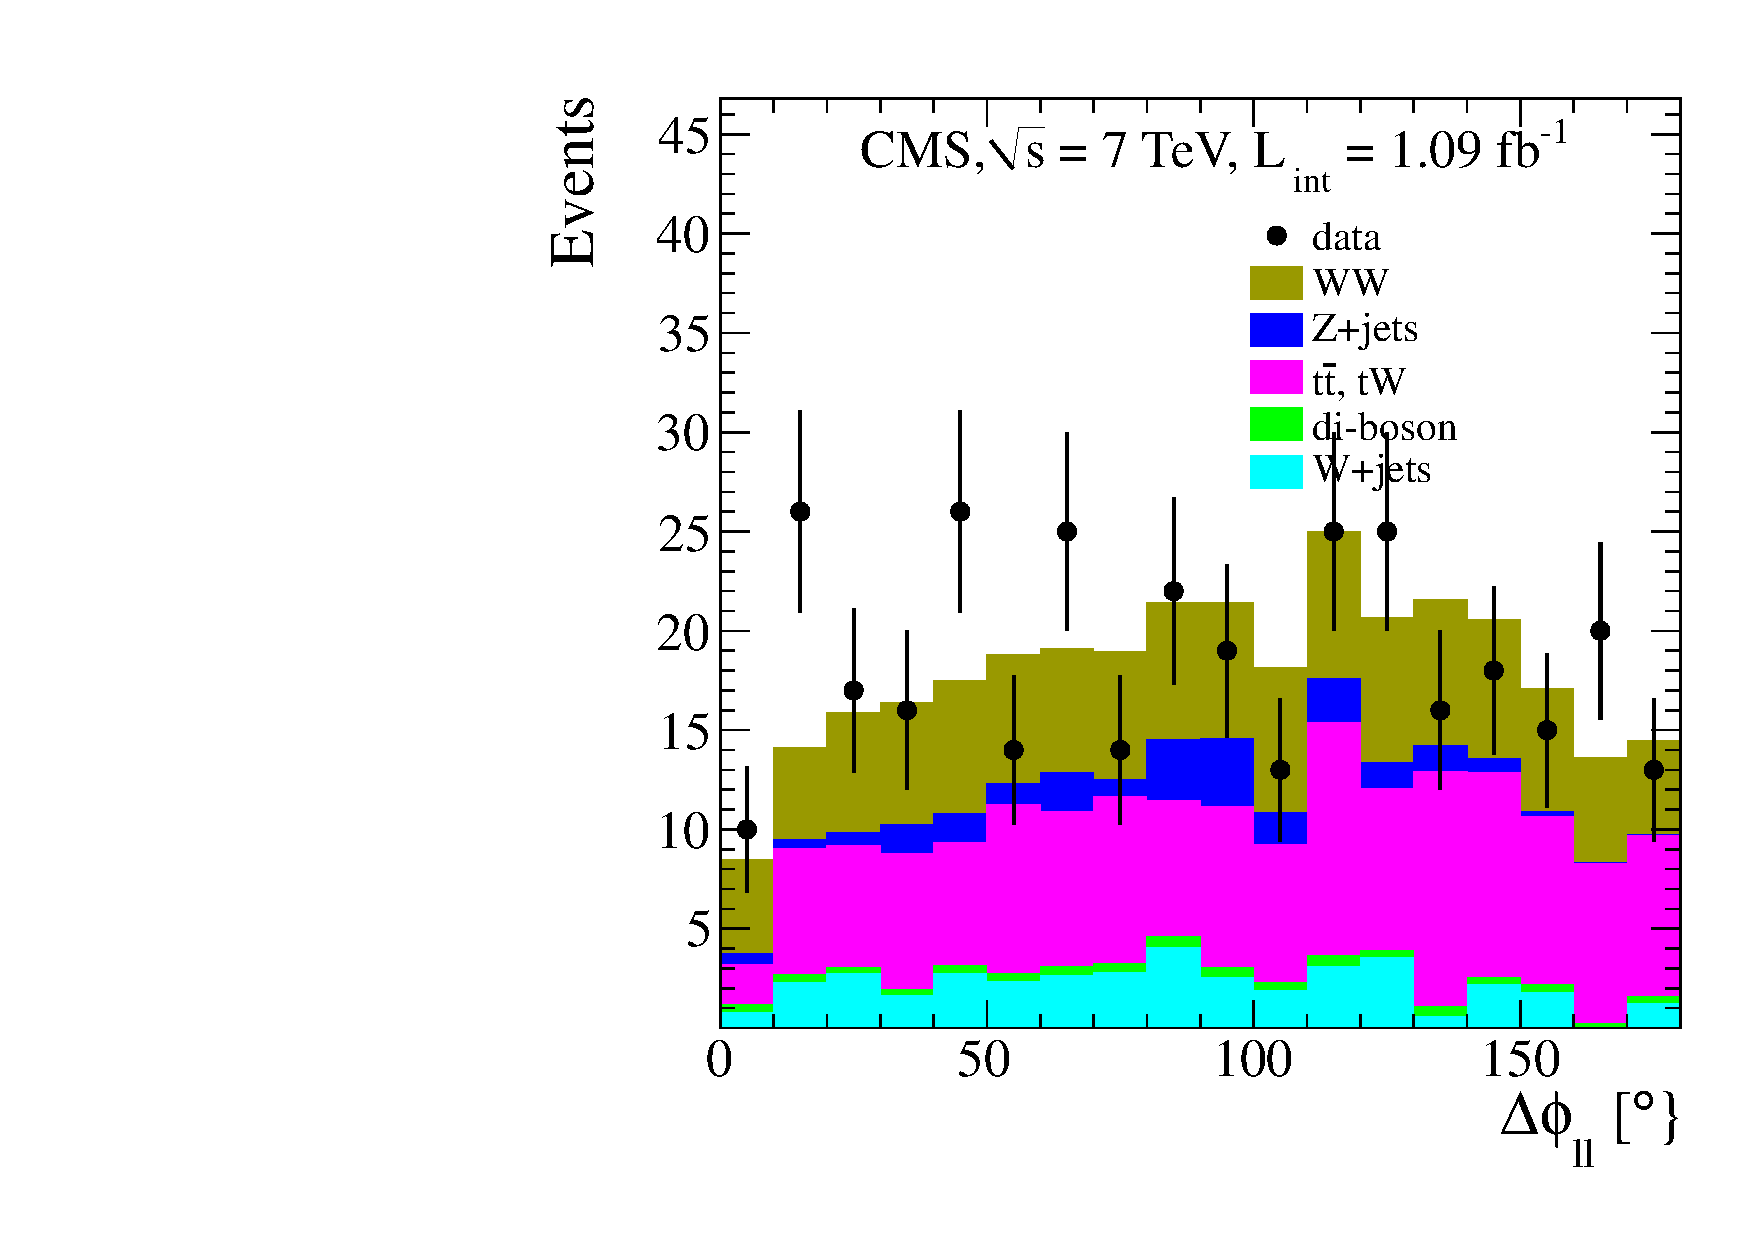
\includegraphics[width=.32\textwidth]{figures/ww_deltaphi_1j.pdf}}
\subfigure[]{
\centering
\label{subfig:ww_deltaphi_2j}
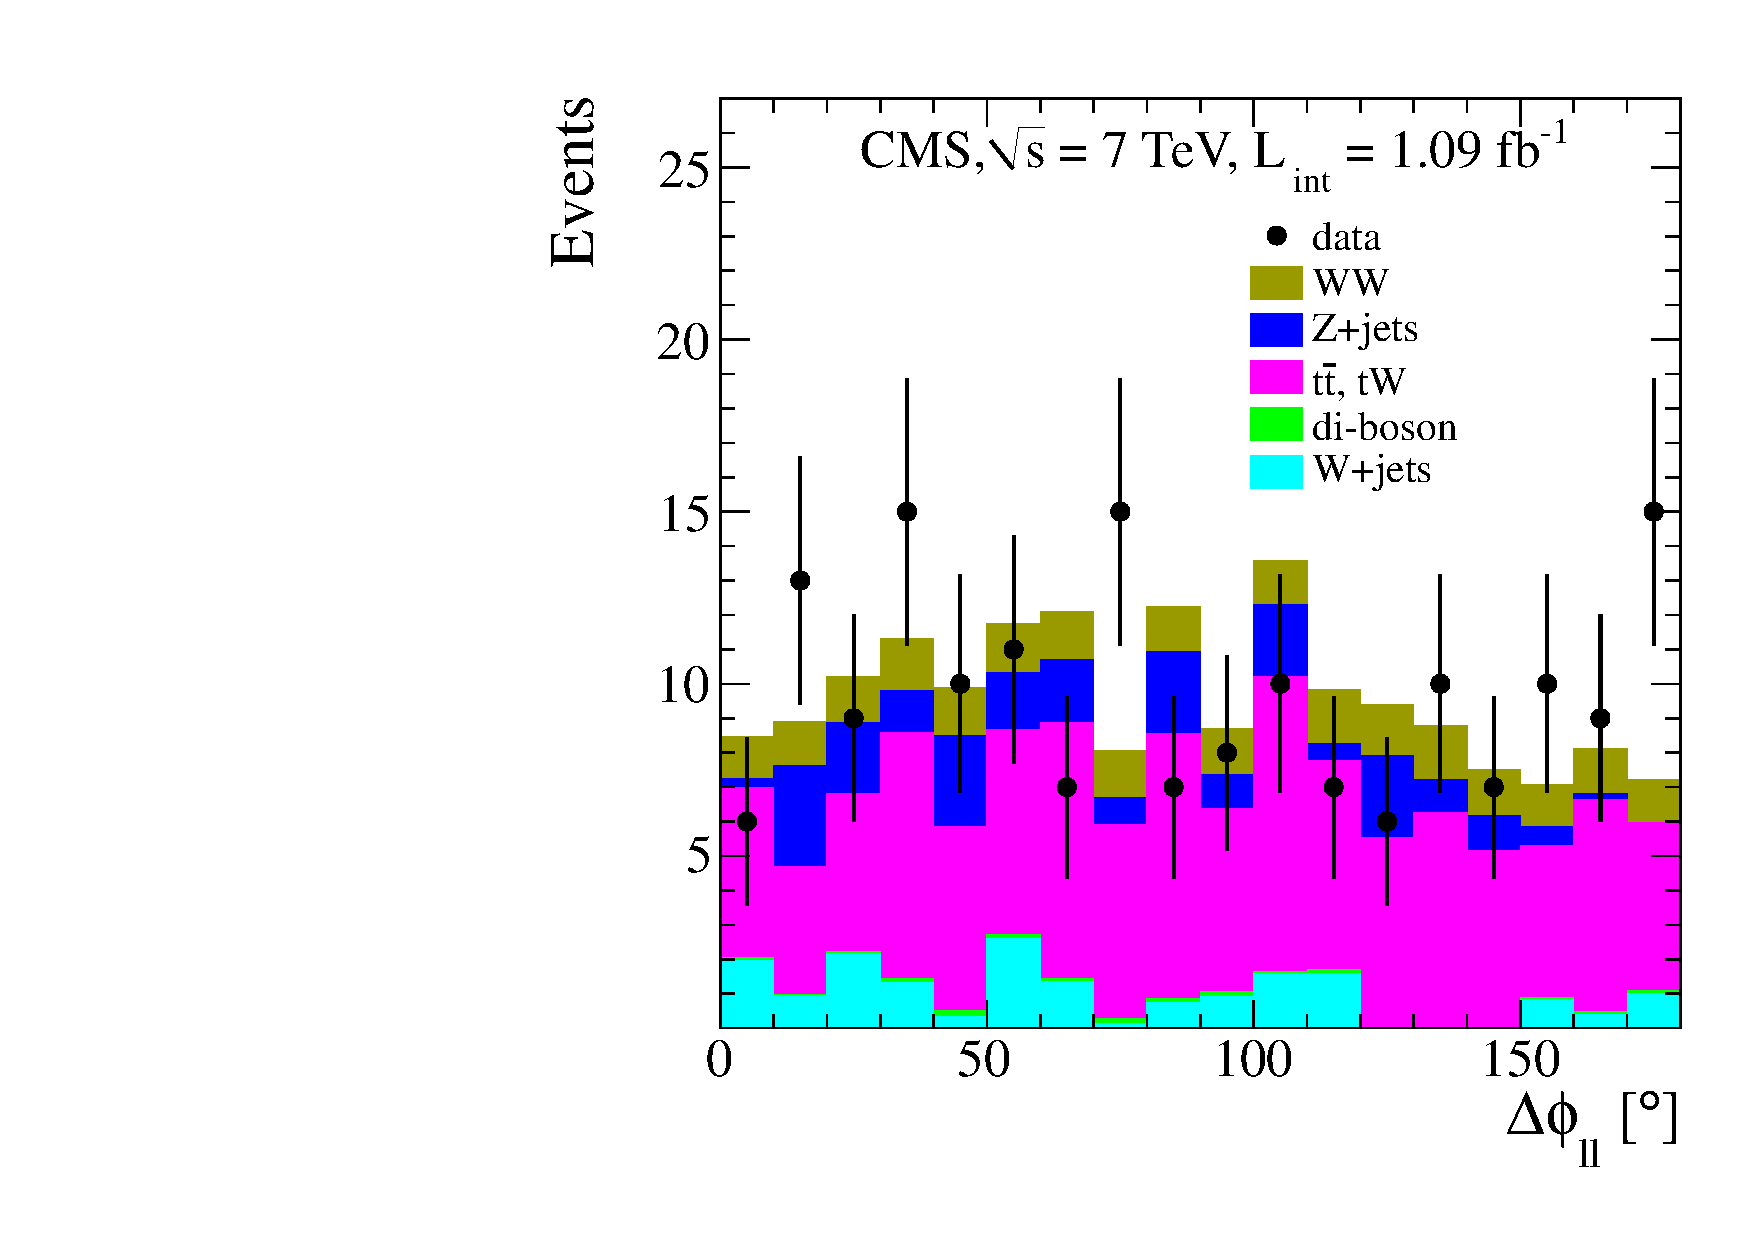
\includegraphics[width=.32\textwidth]{figures/ww_deltaphi_2j.pdf}}\\
\caption{Dilepton $\Delta\phi$ distribution after WW selection for \intlumi of data in the 0-jet \subref{subfig:ww_deltaphi_0j}, 
1-jet \subref{subfig:ww_deltaphi_1j} and 2-jet \subref{subfig:ww_deltaphi_2j} bin analyses. 
MC is scaled to data-driven estimates.}
\label{fig:ww_deltaphi}
\end{figure}

\subsection{$\WW$ Cross-Section Measurement}
As a cross-check, we perform a $\WW$ cross-section measurement using the selected events 
in the 0-jet bin after the $\WW$ preselection. To obtain such a measurement, we take into 
account the background estimation from Section~\ref{sec:backgrounds}, the signal efficiencies 
from Section~\ref{sec:alleff}, and the systematic uncertainties from 
Section~\ref{sec:systematics}. With this information, we obtain a total 
$\WW$ signal efficiency of (6.69 $\pm$  0.62)\% and a background yield of 201.7 $\pm$ 42.4 events, which 
give a total cross section of (55.3 $\pm$   3.3 (stat.) $\pm$   7.6 (syst.) $\pm$   3.3 (lumi.)) pb, 
consistent with the SM expectation of $43 \pm 2$ pb at the $\sim$1 $\sigma$ level.

%\subsection{Background Expectation in the Higgs Regions}

\subsection{Confidence Level Upper Limits}
The cut based and multivariate shape analyses, upper limits at 95\% C.L. are shown 
in Figures~\ref{fig:cutbase_uls_data} and~\ref{fig:mvashape_uls_data}, respectively. 
With \intlumi of data we expect to exclude the Standard Model Higgs in the mass range of
[130,200]~GeV. The observed exclusion range is [150,193]~GeV.
The yields used in data cards of the cut based analysis are shown in
Tables~\ref{tab:cutbase_inputs_of_0j_data}-\ref{tab:cutbase_inputs_2j_data}. 

\begin{figure}[!htbp]
\begin{center}
   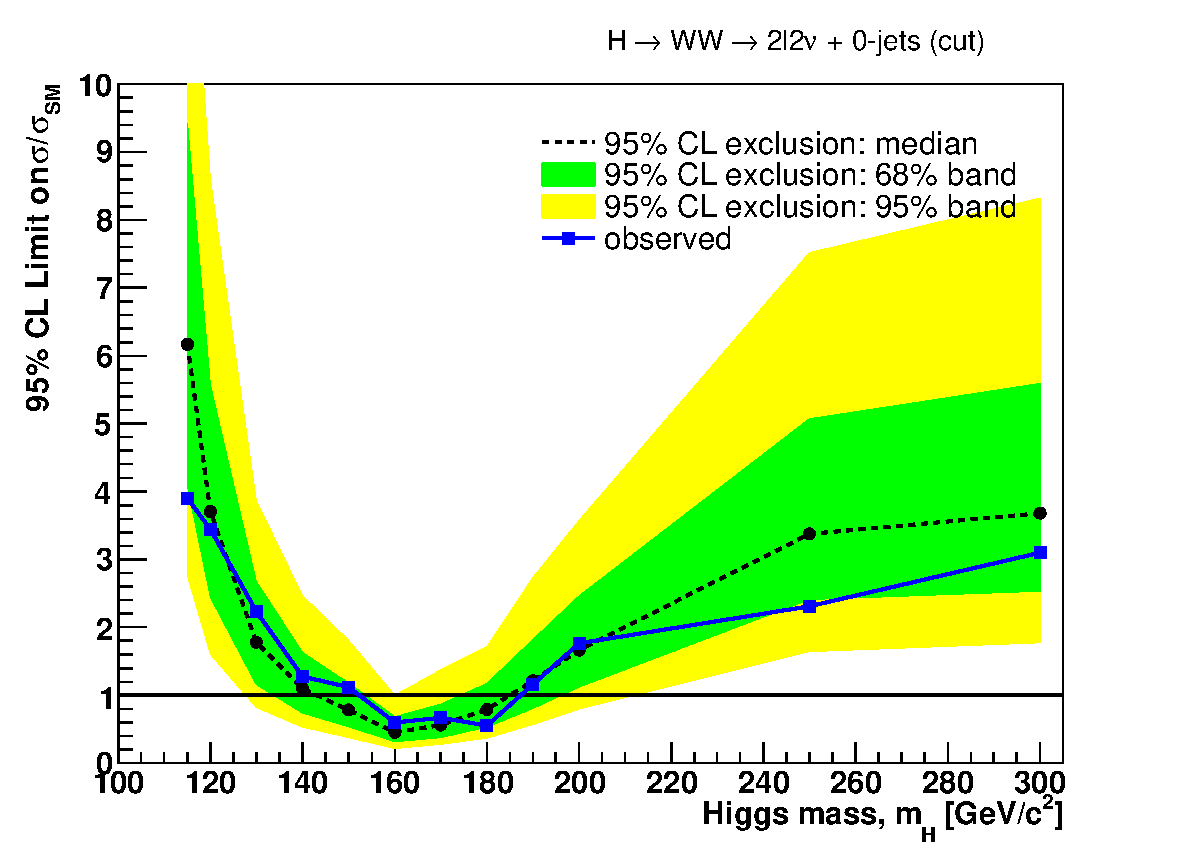
\includegraphics[width=0.49\textwidth]{figures/limits_0j_cut.pdf}
   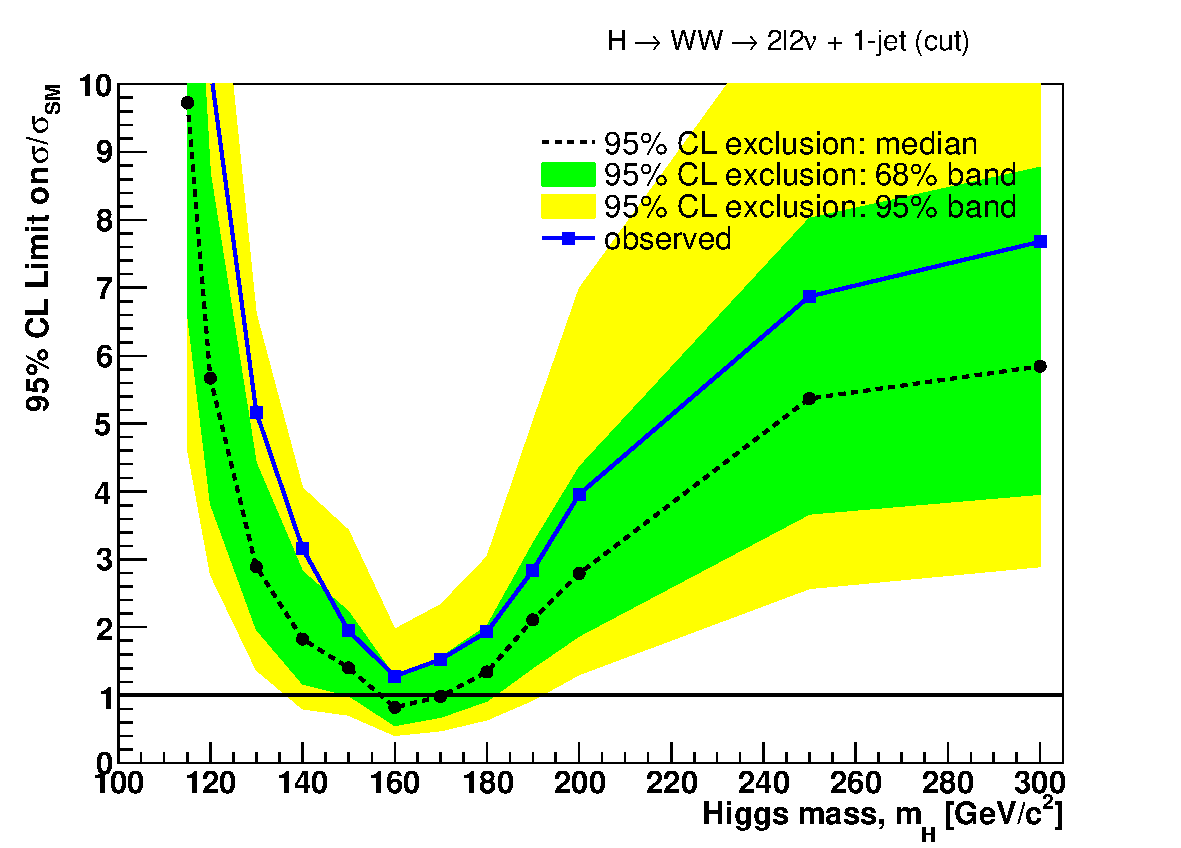
\includegraphics[width=0.49\textwidth]{figures/limits_1j_cut.pdf}
   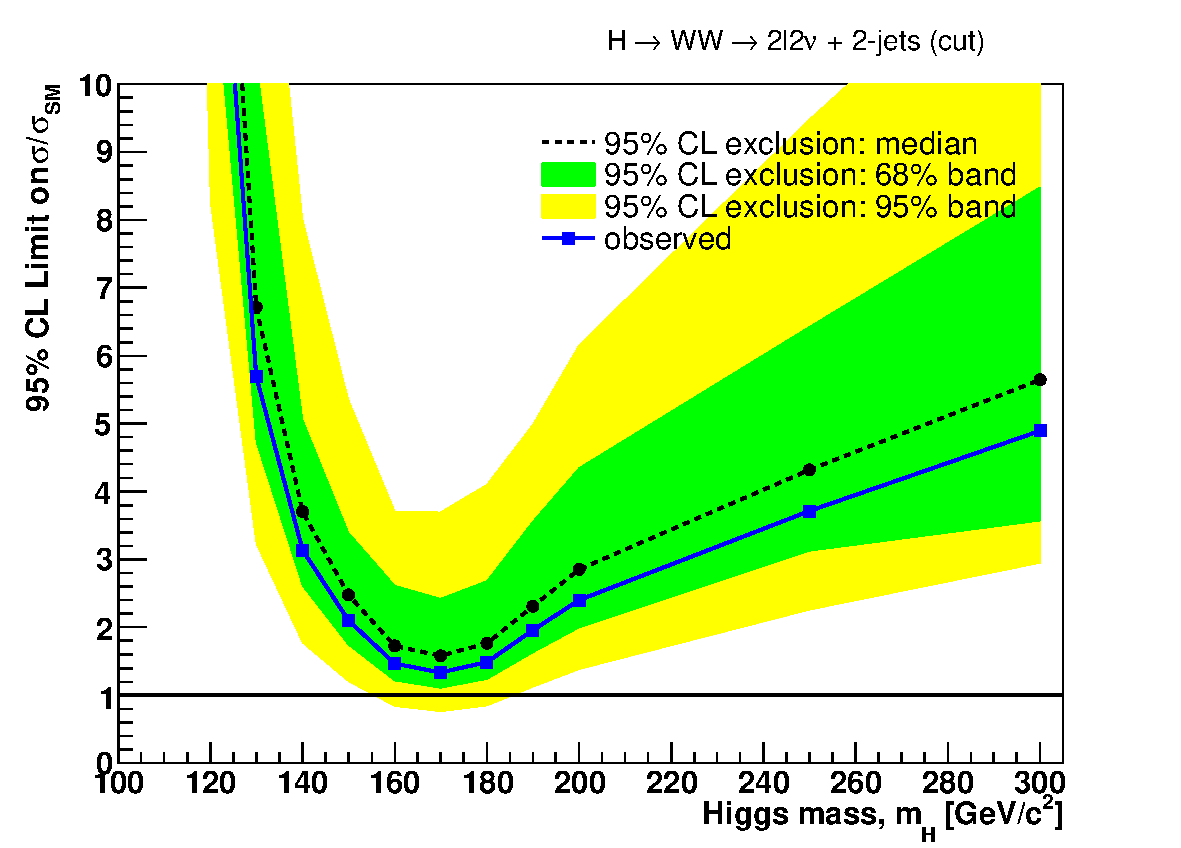
\includegraphics[width=0.49\textwidth]{figures/limits_2j_cut.pdf}
   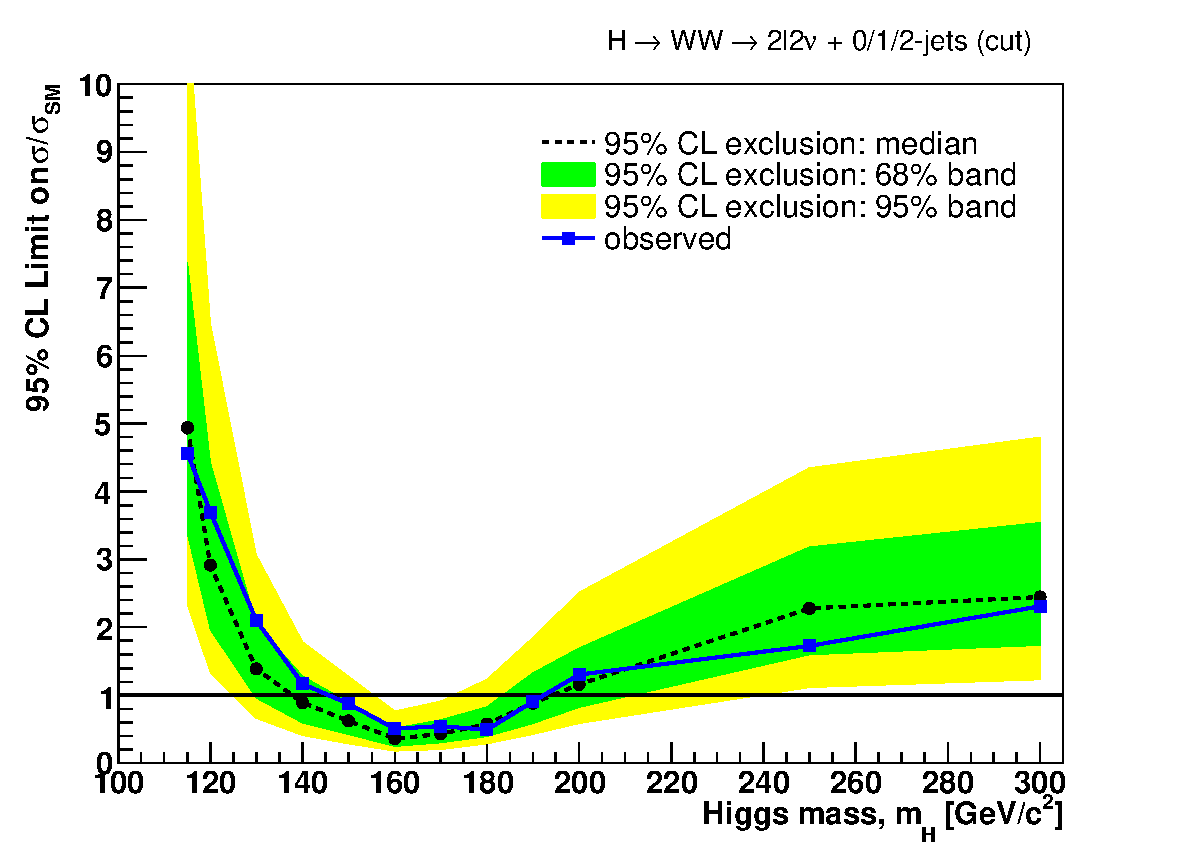
\includegraphics[width=0.49\textwidth]{figures/limits_nj_cut.pdf}
   \caption{Cut based analysis upper limits at 95\% C.L. for \intlumi of data. Top left plot 
   is the result for the 0-jet bin, top right plot is the result for the 1-jet bin, bottom left plot 
   is the result for the 2-jet bin and, bottom right plot is the combined result.}
   \label{fig:cutbase_uls_data}
\end{center}
\end{figure}

%\begin{figure}[!htbp]
%\begin{center}
%   \includegraphics[width=0.49\textwidth]{figures/limits_0j_mva_1.pdf}
%   \includegraphics[width=0.49\textwidth]{figures/limits_1j_mva_1.pdf}
%   \includegraphics[width=0.49\textwidth]{figures/limits_nj_mva_1.pdf}
%   \caption{Multivariate analysis upper limits at 95\% C.L. for \intlumi of data. Top left plot 
%   is the result for the 0-jet bin, top right plot is the result for the 1-jet bin and, 
%   bottom right plot is the combined result.}
%   \label{fig:mvabase_uls_data}
%\end{center}
%\end{figure}

\begin{figure}[!htbp]
\begin{center}
   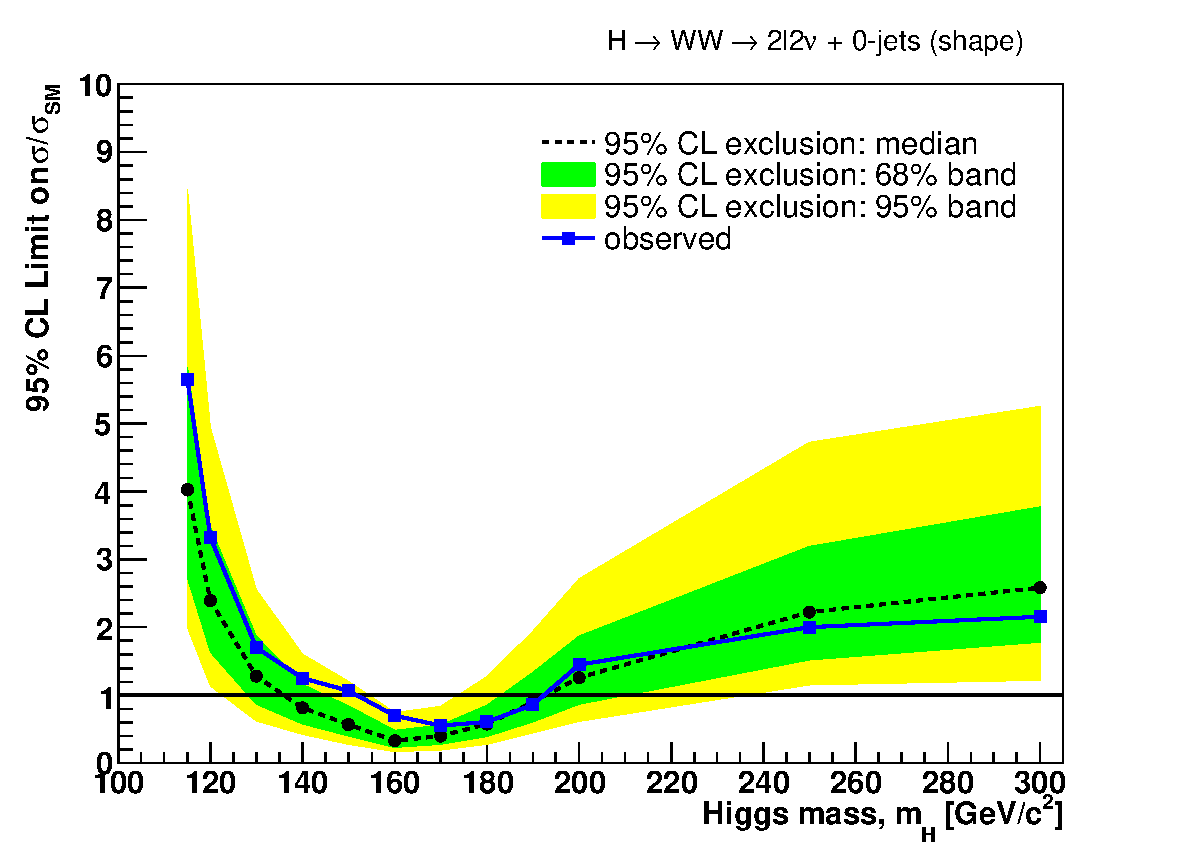
\includegraphics[width=0.49\textwidth]{figures/limits_0j_shape.pdf}
   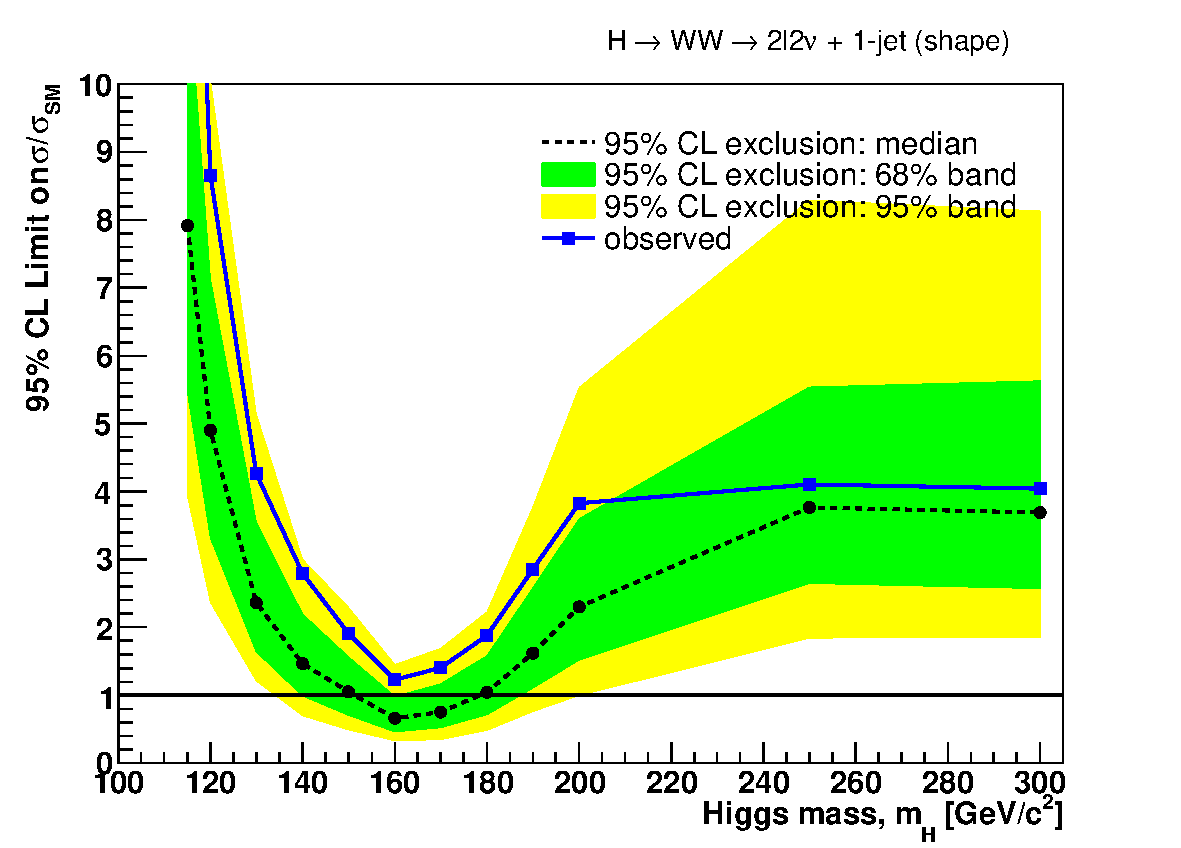
\includegraphics[width=0.49\textwidth]{figures/limits_1j_shape.pdf}
   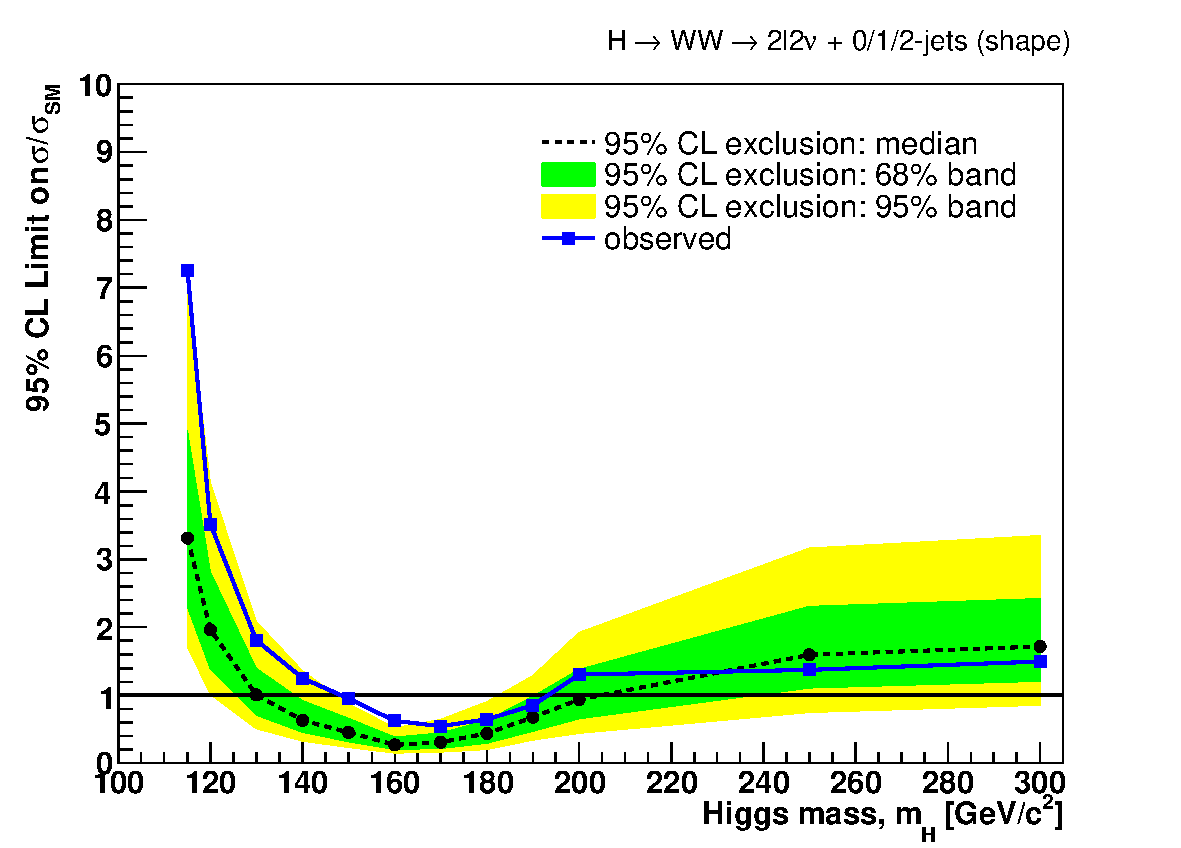
\includegraphics[width=0.49\textwidth]{figures/limits_nj_shape.pdf}
   \caption{Multivariate shape analysis upper limits at 95\% C.L. for \intlumi of data. Top left plot 
   is the result for the 0-jet bin, top right plot is the result for the 1-jet bin and, 
   bottom right plot is the combined result.}
   \label{fig:mvashape_uls_data}
\end{center}
\end{figure}

\begin{table}
{\scriptsize
 \begin{center}
 \begin{tabular}{l| c c c c }
 \hline
Mass     &           Observed &   Median Expected   &      68\% probability band &   95\% probability band \\
 \hline
115  &   4.6  &           4.9 &   [3.4, 7.4]   &    [2.3, 11.2] \\
120  &   3.7  &           2.9 &   [2.0, 4.4]   &    [1.3, 6.5]  \\
130  &   2.1  &           1.4 &   [1.0, 2.0]   &    [0.7, 3.1]  \\
140  &   1.2  &           0.9 &   [0.6, 1.3]   &    [0.4, 1.8]  \\
150  &   0.9  &           0.6 &   [0.4, 0.9]   &    [0.3, 1.3]  \\
160  &   0.5  &           0.4 &   [0.2, 0.5]   &    [0.2, 0.8] \\ 
170  &   0.5  &           0.4 &   [0.3, 0.6]   &    [0.2, 0.9] \\ 
180  &   0.5  &           0.6 &   [0.4, 0.8]   &    [0.3, 1.2] \\ 
190  &   0.9  &           0.9 &   [0.6, 1.3]   &    [0.4, 1.9] \\ 
200  &   1.3  &           1.2 &   [0.8, 1.7]   &    [0.6, 2.5] \\ 
250  &   1.7  &           2.3 &   [1.6, 3.2]   &    [1.1, 4.3] \\ 
300  &   2.3  &           2.4 &   [1.7, 3.5]   &    [1.2, 4.8] \\ 
350  &   2.4  &           2.4 &   [1.6, 3.3]   &    [1.2, 4.6] \\ 
400  &   2.3  &           2.6 &   [1.8, 3.9]   &    [1.3, 5.5] \\ 
450  &   2.3  &           3.6 &   [2.5, 5.2]   &    [1.8, 7.6] \\ 
500  &   3.2  &           4.7 &   [3.3, 7.2]   &    [2.4, 10.1]\\ 
550  &   3.4  &           6.8 &   [4.7, 9.8]   &    [3.3, 13.8]\\ 
600  &   4.5  &           9.4 &   [6.9, 13.4]  &    [5.0, 19.2]\\
\hline
\end{tabular}
\end{center}
}
\caption{Cut based analysis expected and observed Upper Limits with \intlumi of data}
\label{tab:cut_limits_data}
\end{table}

\begin{table}
{\scriptsize
 \begin{center}
 \begin{tabular}{l| c c c c }
 \hline
Mass     &           Observed &   Median Expected   &      68\% probability band &   95\% probability band \\
 \hline
115 &                7.3 &  3.3 &  [2.3, 4.9]  &    [1.7, 7.0] \\
120 &                3.5 &  2.0 &  [1.4, 2.8]  &    [1.0, 4.1] \\
130 &                1.8 &  1.0 &  [0.7, 1.4]  &    [0.5, 2.1] \\
140 &                1.3 &  0.6 &  [0.4, 0.9]  &    [0.3, 1.4] \\
150 &                0.9 &  0.5 &  [0.3, 0.7]  &    [0.2, 0.9] \\
160 &                0.6 &  0.3 &  [0.2, 0.4]  &    [0.1, 0.5]\\
170 &                0.5 &  0.3 &  [0.2, 0.4]  &    [0.2, 0.6]\\
180 &                0.6 &  0.4 &  [0.3, 0.6]  &    [0.2, 0.9]\\
190 &                0.9 &  0.7 &  [0.5, 1.0]  &    [0.3, 1.3]\\
200 &                1.3 &  0.9 &  [0.7, 1.4]  &    [0.4, 1.9]\\
250 &                1.4 &  1.6 &  [1.1, 2.3]  &    [0.7, 3.2]\\
300 &                1.5 &  1.7 &  [1.2, 2.4]  &    [0.9, 3.3]\\
350 &                2.1 &  1.7 &  [1.1, 2.4]  &    [0.8, 3.4]\\
400 &                1.6 &  1.8 &  [1.3, 2.6]  &    [0.9, 3.8]\\
450 &                2.2 &  2.5 &  [1.8, 3.6]  &    [1.3, 5.3]\\
500 &                2.1 &  3.5 &  [2.5, 5.0]  &    [1.9, 6.8]\\
550 &                3.4 &  5.0 &  [3.5, 7.2]  &    [2.6, 9.6]\\
600 &                4.6 &  6.9 &  [5.0, 10.0] &    [3.7, 14.1]\\
 \hline
\end{tabular}
\end{center}
}
\caption{Shape based analysis expected and observed Upper Limits with \intlumi of data}
\label{tab:shape_limits_data}
\end{table}


\begin{table}
{\scriptsize
 \begin{center}
 \begin{tabular}{l c c c c c c c c c c }
 \hline
 Mass & ggH & qqWW & ggWW & VV & Top & Zjets & Wjets & Wgamma & $\sum$Bkg & Data \\
 \hline
115 & $2.8\pm0.7$ & $20.7\pm3.6$ & $0.8\pm0.4$ & $0.5\pm0.1$ & $2.1\pm0.8$ & $0.1\pm0.0$ & $15.3\pm5.9$ & $2.7\pm0.8$ & $42.2\pm7.0$ & 42 \\
120 & $5.4\pm1.2$ & $25.3\pm4.4$ & $1.1\pm0.6$ & $0.6\pm0.1$ & $2.7\pm1.0$ & $0.1\pm0.0$ & $15.8\pm6.1$ & $2.7\pm0.8$ & $48.3\pm7.7$ & 51 \\
130 & $10.0\pm2.3$ & $27.3\pm4.8$ & $1.3\pm0.7$ & $0.6\pm0.1$ & $2.7\pm1.0$ & $0.1\pm0.0$ & $11.2\pm4.4$ & $1.4\pm0.6$ & $44.6\pm6.7$ & 52 \\
140 & $13.3\pm3.0$ & $23.2\pm4.1$ & $1.2\pm0.6$ & $0.5\pm0.1$ & $2.7\pm1.0$ & $0.0\pm0.0$ & $5.3\pm2.3$ & $1.0\pm0.5$ & $34.1\pm4.9$ & 37 \\
150 & $12.5\pm2.9$ & $14.6\pm2.6$ & $1.1\pm0.6$ & $0.3\pm0.1$ & $2.1\pm0.9$ & $0.0\pm0.0$ & $2.4\pm1.4$ & $0.3\pm0.3$ & $20.8\pm3.1$ & 20 \\
160 & $18.8\pm4.4$ & $9.8\pm1.7$ & $1.0\pm0.5$ & $0.2\pm0.1$ & $1.6\pm0.8$ & $0.0\pm0.0$ & $1.9\pm1.2$ & $0.0\pm0.0$ & $14.5\pm2.3$ & 15 \\
170 & $14.3\pm3.4$ & $7.5\pm1.3$ & $1.0\pm0.5$ & $0.2\pm0.0$ & $1.1\pm0.6$ & $0.0\pm0.0$ & $1.7\pm1.1$ & $0.0\pm0.0$ & $11.5\pm1.9$ & 13 \\
180 & $10.8\pm2.5$ & $8.7\pm1.5$ & $1.2\pm0.6$ & $0.2\pm0.1$ & $1.9\pm0.9$ & $0.0\pm0.0$ & $1.2\pm0.9$ & $0.0\pm0.0$ & $13.3\pm2.1$ & 14 \\
190 & $9.5\pm2.3$ & $13.6\pm2.4$ & $1.6\pm0.9$ & $0.3\pm0.1$ & $3.2\pm1.3$ & $0.0\pm0.0$ & $1.4\pm0.9$ & $0.0\pm0.0$ & $20.2\pm3.0$ & 22 \\
200 & $6.9\pm1.7$ & $14.7\pm2.6$ & $1.7\pm0.9$ & $0.4\pm0.1$ & $4.1\pm1.5$ & $0.0\pm0.0$ & $1.3\pm0.9$ & $0.0\pm0.0$ & $22.2\pm3.2$ & 26 \\
250 & $3.6\pm0.9$ & $13.4\pm2.4$ & $1.3\pm0.7$ & $0.5\pm0.1$ & $7.6\pm2.4$ & $0.0\pm0.0$ & $1.2\pm0.7$ & $0.0\pm0.0$ & $24.0\pm3.5$ & 21 \\
300 & $2.8\pm0.8$ & $11.4\pm2.0$ & $1.0\pm0.5$ & $0.3\pm0.1$ & $4.6\pm1.5$ & $0.0\pm0.0$ & $0.9\pm0.5$ & $0.2\pm0.2$ & $18.4\pm2.6$ & 17 \\
350 & $2.9\pm0.9$ & $9.7\pm1.7$ & $0.8\pm0.4$ & $0.2\pm0.1$ & $4.2\pm1.4$ & $0.0\pm0.0$ & $0.9\pm0.5$ & $0.2\pm0.2$ & $16.1\pm2.3$ & 15 \\
400 & $2.4\pm0.7$ & $7.9\pm1.4$ & $0.7\pm0.4$ & $0.2\pm0.1$ & $4.7\pm1.7$ & $0.0\pm0.0$ & $0.5\pm0.4$ & $0.2\pm0.2$ & $14.2\pm2.2$ & 12 \\
450 & $1.3\pm0.4$ & $4.7\pm0.8$ & $0.4\pm0.2$ & $0.1\pm0.0$ & $3.1\pm1.2$ & $0.0\pm0.0$ & $0.8\pm0.5$ & $0.0\pm0.0$ & $9.1\pm1.6$ & 6 \\
500 & $0.9\pm0.3$ & $3.8\pm0.7$ & $0.4\pm0.2$ & $0.1\pm0.0$ & $2.7\pm1.1$ & $0.0\pm0.0$ & $0.8\pm0.5$ & $0.0\pm0.0$ & $7.8\pm1.4$ & 4 \\
550 & $0.5\pm0.2$ & $2.9\pm0.5$ & $0.3\pm0.2$ & $0.1\pm0.0$ & $1.9\pm0.9$ & $0.0\pm0.0$ & $0.8\pm0.5$ & $0.0\pm0.0$ & $6.0\pm1.2$ & 2 \\
600 & $0.3\pm0.1$ & $2.4\pm0.4$ & $0.2\pm0.1$ & $0.1\pm0.0$ & $1.3\pm0.7$ & $0.0\pm0.0$ & $0.6\pm0.4$ & $0.0\pm0.0$ & $4.6\pm0.9$ & 1 \\
\hline
\end{tabular}
\end{center}
}
\caption{Cut based analysis expected and observed yields for 0-jet case with \intlumi of data for opposite-flavor events}
\label{tab:cutbase_inputs_of_0j_data}
\end{table}

\begin{table}
{\scriptsize
 \begin{center}
 \begin{tabular}{l c c c c c c c c c c }
 \hline
 Mass & ggH & qqWW & ggWW & VV & Top & Zjets & Wjets & Wgamma & $\sum$Bkg & Data \\
 \hline
115 & $1.8\pm0.4$ & $13.0\pm2.3$ & $0.5\pm0.3$ & $0.2\pm0.1$ & $0.9\pm0.5$ & $3.2\pm7.2$ & $6.6\pm2.8$ & $0.1\pm0.1$ & $24.5\pm8.1$ & 15 \\
120 & $3.7\pm0.9$ & $18.5\pm3.2$ & $0.8\pm0.4$ & $0.3\pm0.1$ & $1.2\pm0.6$ & $4.0\pm9.0$ & $7.8\pm3.2$ & $0.1\pm0.1$ & $32.9\pm10.1$ & 31 \\
130 & $8.2\pm1.9$ & $22.8\pm4.0$ & $1.1\pm0.6$ & $0.4\pm0.1$ & $0.9\pm0.4$ & $1.5\pm2.9$ & $7.5\pm3.1$ & $0.1\pm0.1$ & $34.4\pm5.9$ & 39 \\
140 & $11.2\pm2.6$ & $21.5\pm3.8$ & $1.1\pm0.6$ & $0.3\pm0.1$ & $1.2\pm0.4$ & $1.0\pm1.7$ & $4.7\pm2.1$ & $0.0\pm0.0$ & $29.8\pm4.7$ & 33 \\
150 & $12.1\pm2.8$ & $13.3\pm2.3$ & $1.0\pm0.5$ & $0.3\pm0.1$ & $0.7\pm0.4$ & $0.8\pm2.0$ & $0.2\pm0.4$ & $0.0\pm0.0$ & $16.4\pm3.2$ & 26 \\
160 & $17.5\pm4.1$ & $9.2\pm1.6$ & $0.9\pm0.5$ & $0.3\pm0.1$ & $1.1\pm0.6$ & $1.6\pm2.8$ & $0.0\pm0.2$ & $0.0\pm0.0$ & $13.1\pm3.3$ & 19 \\
170 & $14.6\pm3.4$ & $7.3\pm1.3$ & $0.9\pm0.5$ & $0.3\pm0.1$ & $1.5\pm0.8$ & $3.8\pm6.9$ & $0.0\pm0.0$ & $0.0\pm0.0$ & $13.7\pm7.1$ & 16 \\
180 & $10.4\pm2.5$ & $8.1\pm1.4$ & $1.1\pm0.6$ & $0.2\pm0.1$ & $2.6\pm1.1$ & $0.7\pm3.6$ & $0.0\pm0.0$ & $0.0\pm0.0$ & $12.7\pm4.0$ & 8 \\
190 & $8.3\pm2.0$ & $11.8\pm2.1$ & $1.6\pm0.8$ & $0.3\pm0.1$ & $3.6\pm1.4$ & $3.4\pm4.9$ & $0.6\pm0.6$ & $0.0\pm0.0$ & $21.2\pm5.6$ & 20 \\
200 & $5.5\pm1.3$ & $11.4\pm2.0$ & $1.5\pm0.8$ & $0.3\pm0.1$ & $3.4\pm1.3$ & $1.7\pm2.0$ & $1.0\pm0.7$ & $0.0\pm0.0$ & $19.3\pm3.3$ & 18 \\
250 & $2.0\pm0.5$ & $7.9\pm1.4$ & $0.9\pm0.5$ & $0.3\pm0.1$ & $4.6\pm1.6$ & $1.0\pm0.3$ & $2.0\pm1.1$ & $0.0\pm0.0$ & $16.6\pm2.5$ & 11 \\
300 & $2.1\pm0.6$ & $7.6\pm1.3$ & $0.7\pm0.4$ & $0.2\pm0.1$ & $4.8\pm1.6$ & $0.9\pm0.4$ & $1.5\pm0.8$ & $0.0\pm0.0$ & $15.6\pm2.3$ & 14 \\
350 & $2.3\pm0.7$ & $7.2\pm1.3$ & $0.6\pm0.3$ & $0.3\pm0.1$ & $4.2\pm1.5$ & $0.7\pm0.1$ & $1.3\pm0.8$ & $0.0\pm0.0$ & $14.2\pm2.1$ & 11 \\
400 & $1.8\pm0.5$ & $5.9\pm1.1$ & $0.5\pm0.2$ & $0.2\pm0.1$ & $3.4\pm1.2$ & $0.6\pm0.1$ & $1.2\pm0.7$ & $0.0\pm0.0$ & $11.8\pm1.8$ & 10 \\
450 & $1.0\pm0.3$ & $3.3\pm0.6$ & $0.3\pm0.1$ & $0.2\pm0.0$ & $3.2\pm1.2$ & $0.3\pm0.1$ & $0.9\pm0.6$ & $0.0\pm0.0$ & $8.2\pm1.5$ & 5 \\
500 & $0.6\pm0.2$ & $2.6\pm0.5$ & $0.2\pm0.1$ & $0.1\pm0.0$ & $2.2\pm0.9$ & $0.2\pm0.0$ & $0.4\pm0.3$ & $0.0\pm0.0$ & $5.8\pm1.1$ & 3 \\
550 & $0.4\pm0.1$ & $2.1\pm0.4$ & $0.2\pm0.1$ & $0.1\pm0.0$ & $1.7\pm0.7$ & $0.2\pm0.0$ & $0.3\pm0.2$ & $0.0\pm0.0$ & $4.5\pm0.9$ & 2 \\
600 & $0.2\pm0.1$ & $1.7\pm0.3$ & $0.1\pm0.1$ & $0.0\pm0.0$ & $1.4\pm0.6$ & $0.2\pm0.0$ & $0.3\pm0.2$ & $0.0\pm0.0$ & $3.7\pm0.8$ & 1 \\
\hline
\end{tabular}
\end{center}
}
\caption{Cut based analysis expected and observed yields for 0-jet case with \intlumi of data for same-flavor events}
\label{tab:cutbase_inputs_sf_0j_data}
\end{table}
\begin{table}
{\scriptsize
 \begin{center}
 \begin{tabular}{l c c c c c c c c c c }
 \hline
 Mass & ggH & qqWW & ggWW & VV & Top & Zjets & Wjets & Wgamma & $\sum$Bkg & Data \\
 \hline
115 & $0.9\pm0.3$ & $5.3\pm2.0$ & $0.3\pm0.2$ & $0.5\pm0.1$ & $4.2\pm1.0$ & $0.0\pm0.0$ & $2.4\pm1.3$ & $0.2\pm0.2$ & $12.9\pm2.6$ & 21 \\
120 & $1.7\pm0.6$ & $6.6\pm2.5$ & $0.4\pm0.3$ & $0.5\pm0.1$ & $4.8\pm1.0$ & $0.1\pm0.0$ & $2.9\pm1.4$ & $0.2\pm0.2$ & $15.6\pm3.1$ & 23 \\
130 & $3.4\pm1.2$ & $7.4\pm2.8$ & $0.5\pm0.3$ & $0.5\pm0.1$ & $6.1\pm1.2$ & $0.4\pm0.3$ & $3.3\pm1.6$ & $0.0\pm0.0$ & $18.2\pm3.4$ & 22 \\
140 & $4.7\pm1.6$ & $6.5\pm2.4$ & $0.5\pm0.3$ & $0.4\pm0.1$ & $5.1\pm1.1$ & $0.4\pm0.3$ & $2.0\pm1.1$ & $0.0\pm0.0$ & $14.9\pm2.9$ & 16 \\
150 & $5.4\pm1.8$ & $5.6\pm2.1$ & $0.5\pm0.3$ & $0.3\pm0.1$ & $4.7\pm1.0$ & $0.2\pm0.1$ & $0.9\pm0.5$ & $0.0\pm0.0$ & $12.1\pm2.4$ & 11 \\
160 & $8.0\pm2.6$ & $4.5\pm1.7$ & $0.5\pm0.3$ & $0.2\pm0.1$ & $4.0\pm0.9$ & $0.0\pm0.0$ & $0.5\pm0.4$ & $0.0\pm0.0$ & $9.6\pm2.0$ & 9 \\
170 & $5.9\pm1.9$ & $3.6\pm1.4$ & $0.4\pm0.2$ & $0.1\pm0.0$ & $3.6\pm0.9$ & $0.0\pm0.0$ & $0.1\pm0.2$ & $0.0\pm0.0$ & $7.9\pm1.7$ & 7 \\
180 & $4.6\pm1.5$ & $4.3\pm1.6$ & $0.5\pm0.3$ & $0.1\pm0.0$ & $3.7\pm0.9$ & $0.0\pm0.0$ & $0.2\pm0.3$ & $0.0\pm0.0$ & $8.9\pm1.9$ & 9 \\
190 & $3.9\pm1.3$ & $6.3\pm2.4$ & $0.7\pm0.4$ & $0.2\pm0.1$ & $8.1\pm1.6$ & $0.0\pm0.0$ & $0.9\pm0.6$ & $0.0\pm0.0$ & $16.2\pm3.0$ & 15 \\
200 & $3.2\pm1.0$ & $7.5\pm2.8$ & $0.8\pm0.5$ & $0.3\pm0.1$ & $9.3\pm1.7$ & $0.0\pm0.0$ & $1.3\pm0.8$ & $0.0\pm0.0$ & $19.2\pm3.4$ & 19 \\
250 & $2.0\pm0.6$ & $7.7\pm2.9$ & $0.6\pm0.4$ & $0.4\pm0.1$ & $15.4\pm2.5$ & $0.0\pm0.0$ & $1.8\pm1.0$ & $0.0\pm0.0$ & $26.0\pm4.0$ & 27 \\
300 & $1.7\pm0.6$ & $7.2\pm2.7$ & $0.5\pm0.3$ & $0.3\pm0.1$ & $13.5\pm2.3$ & $0.1\pm0.1$ & $1.0\pm0.8$ & $0.0\pm0.0$ & $22.7\pm3.6$ & 25 \\
350 & $1.8\pm0.6$ & $6.4\pm2.4$ & $0.4\pm0.3$ & $0.3\pm0.1$ & $11.9\pm2.1$ & $0.1\pm0.1$ & $0.9\pm0.7$ & $0.0\pm0.0$ & $20.0\pm3.3$ & 22 \\
400 & $1.6\pm0.5$ & $5.4\pm2.1$ & $0.3\pm0.2$ & $0.3\pm0.1$ & $12.0\pm2.1$ & $0.1\pm0.1$ & $0.6\pm0.6$ & $0.0\pm0.0$ & $18.7\pm3.0$ & 17 \\
450 & $1.0\pm0.3$ & $3.5\pm1.3$ & $0.2\pm0.1$ & $0.1\pm0.0$ & $6.8\pm1.5$ & $0.1\pm0.1$ & $0.3\pm0.4$ & $0.0\pm0.0$ & $11.1\pm2.0$ & 9 \\
500 & $0.6\pm0.2$ & $2.7\pm1.0$ & $0.2\pm0.1$ & $0.1\pm0.0$ & $4.5\pm1.1$ & $0.1\pm0.1$ & $0.3\pm0.4$ & $0.0\pm0.0$ & $7.9\pm1.6$ & 8 \\
550 & $0.4\pm0.1$ & $2.3\pm0.9$ & $0.1\pm0.1$ & $0.1\pm0.0$ & $4.2\pm1.1$ & $0.1\pm0.1$ & $0.5\pm0.4$ & $0.0\pm0.0$ & $7.3\pm1.5$ & 5 \\
600 & $0.3\pm0.1$ & $1.8\pm0.7$ & $0.1\pm0.1$ & $0.1\pm0.0$ & $3.1\pm0.9$ & $0.1\pm0.1$ & $0.5\pm0.4$ & $0.0\pm0.0$ & $5.7\pm1.2$ & 4 \\
\hline
\end{tabular}
\end{center}
}
\caption{Cut based analysis expected and observed yields for 1-jet case with \intlumi of data for opposite-flavor events}
\label{tab:cutbase_inputs_of_1j_data}
\end{table}

\begin{table}
{\scriptsize
 \begin{center}
 \begin{tabular}{l c c c c c c c c c c }
 \hline
 Mass & ggH & qqWW & ggWW & VV & Top & Zjets & Wjets & Wgamma & $\sum$Bkg & Data \\
 \hline
115 & $0.5\pm0.2$ & $2.8\pm1.0$ & $0.1\pm0.1$ & $0.2\pm0.0$ & $1.9\pm0.7$ & $0.7\pm2.1$ & $2.3\pm1.3$ & $0.2\pm0.2$ & $8.1\pm2.8$ & 10 \\
120 & $1.0\pm0.3$ & $4.0\pm1.5$ & $0.2\pm0.1$ & $0.2\pm0.1$ & $2.8\pm0.9$ & $1.3\pm4.0$ & $2.4\pm1.4$ & $0.2\pm0.2$ & $11.1\pm4.6$ & 17 \\
130 & $2.1\pm0.7$ & $4.8\pm1.8$ & $0.3\pm0.2$ & $0.2\pm0.1$ & $2.7\pm0.8$ & $0.6\pm1.6$ & $1.9\pm1.2$ & $0.2\pm0.2$ & $10.8\pm2.8$ & 21 \\
140 & $3.2\pm1.1$ & $4.5\pm1.7$ & $0.3\pm0.2$ & $0.2\pm0.1$ & $2.9\pm0.8$ & $0.6\pm1.0$ & $1.4\pm1.0$ & $0.2\pm0.2$ & $10.0\pm2.4$ & 21 \\
150 & $3.9\pm1.3$ & $4.2\pm1.6$ & $0.4\pm0.2$ & $0.1\pm0.0$ & $2.0\pm0.5$ & $1.0\pm2.0$ & $0.8\pm0.7$ & $0.0\pm0.0$ & $8.6\pm2.7$ & 17 \\
160 & $6.3\pm2.1$ & $3.6\pm1.4$ & $0.4\pm0.2$ & $0.1\pm0.0$ & $1.7\pm0.5$ & $0.8\pm1.3$ & $0.8\pm0.7$ & $0.0\pm0.0$ & $7.4\pm2.1$ & 16 \\
170 & $5.1\pm1.7$ & $3.2\pm1.2$ & $0.4\pm0.2$ & $0.1\pm0.0$ & $2.4\pm0.6$ & $0.8\pm1.0$ & $0.2\pm0.4$ & $0.0\pm0.0$ & $7.1\pm1.8$ & 15 \\
180 & $4.2\pm1.4$ & $3.7\pm1.4$ & $0.4\pm0.2$ & $0.1\pm0.0$ & $2.9\pm0.7$ & $0.6\pm0.7$ & $0.1\pm0.4$ & $0.0\pm0.0$ & $7.9\pm1.8$ & 14 \\
190 & $3.5\pm1.1$ & $5.4\pm2.0$ & $0.5\pm0.3$ & $0.1\pm0.0$ & $3.8\pm0.9$ & $1.0\pm1.4$ & $0.0\pm0.4$ & $0.0\pm0.0$ & $10.9\pm2.7$ & 19 \\
200 & $2.3\pm0.7$ & $5.5\pm2.1$ & $0.5\pm0.3$ & $0.1\pm0.0$ & $4.1\pm1.0$ & $1.2\pm1.3$ & $0.5\pm0.6$ & $0.0\pm0.0$ & $12.0\pm2.7$ & 20 \\
250 & $1.0\pm0.3$ & $4.1\pm1.6$ & $0.3\pm0.2$ & $0.2\pm0.0$ & $5.6\pm1.3$ & $1.6\pm0.7$ & $0.0\pm0.0$ & $0.0\pm0.0$ & $11.8\pm2.1$ & 16 \\
300 & $1.1\pm0.4$ & $4.0\pm1.5$ & $0.2\pm0.1$ & $0.1\pm0.0$ & $8.6\pm1.7$ & $0.9\pm1.0$ & $0.1\pm0.3$ & $0.0\pm0.0$ & $13.9\pm2.5$ & 18 \\
350 & $1.3\pm0.4$ & $3.5\pm1.3$ & $0.2\pm0.1$ & $0.1\pm0.0$ & $7.0\pm1.5$ & $0.6\pm0.4$ & $0.2\pm0.4$ & $0.0\pm0.0$ & $11.7\pm2.1$ & 19 \\
400 & $1.1\pm0.4$ & $3.0\pm1.1$ & $0.2\pm0.1$ & $0.1\pm0.0$ & $6.0\pm1.4$ & $0.6\pm0.4$ & $0.2\pm0.4$ & $0.0\pm0.0$ & $10.1\pm1.9$ & 15 \\
450 & $0.6\pm0.2$ & $1.7\pm0.7$ & $0.1\pm0.1$ & $0.0\pm0.0$ & $3.5\pm1.0$ & $0.2\pm0.0$ & $0.3\pm0.4$ & $0.0\pm0.0$ & $5.9\pm1.3$ & 8 \\
500 & $0.5\pm0.1$ & $1.5\pm0.6$ & $0.1\pm0.1$ & $0.0\pm0.0$ & $2.7\pm0.9$ & $0.1\pm0.0$ & $0.2\pm0.3$ & $0.0\pm0.0$ & $4.6\pm1.1$ & 6 \\
550 & $0.3\pm0.1$ & $1.3\pm0.5$ & $0.1\pm0.1$ & $0.0\pm0.0$ & $1.7\pm0.6$ & $0.1\pm0.0$ & $0.3\pm0.3$ & $0.0\pm0.0$ & $3.4\pm0.9$ & 3 \\
600 & $0.2\pm0.1$ & $1.0\pm0.4$ & $0.1\pm0.0$ & $0.0\pm0.0$ & $1.6\pm0.6$ & $0.1\pm0.0$ & $0.1\pm0.3$ & $0.0\pm0.0$ & $2.9\pm0.8$ & 2 \\
\hline
\end{tabular}
\end{center}
}
\caption{Cut based analysis expected and observed yields for 1-jet case with \intlumi of data for same-flavor events}
\label{tab:cutbase_inputs_sf_1j_data}
\end{table}

\begin{table}
{\scriptsize
 \begin{center}
 \begin{tabular}{l c c c c c c c c c c }
 \hline
 Mass & ggH & qqWW & ggWW & VV & Top & Zjets & Wjets & Wgamma & $\sum$Bkg & Data \\
 \hline
115 & $0.0\pm0.0$ & $0.3\pm0.1$ & $0.1\pm0.0$ & $0.0\pm0.0$ & $1.8\pm1.1$ & $0.6\pm0.6$ & $0.5\pm0.4$ & $0.0\pm0.0$ & $3.3\pm1.3$ & 3 \\
120 & $0.1\pm0.0$ & $0.3\pm0.1$ & $0.1\pm0.0$ & $0.0\pm0.0$ & $1.8\pm1.1$ & $0.6\pm0.6$ & $0.5\pm0.4$ & $0.0\pm0.0$ & $3.3\pm1.3$ & 3 \\
130 & $0.2\pm0.1$ & $0.4\pm0.1$ & $0.1\pm0.0$ & $0.0\pm0.0$ & $1.9\pm1.1$ & $0.6\pm0.6$ & $0.5\pm0.4$ & $0.0\pm0.0$ & $3.4\pm1.3$ & 3 \\
140 & $0.3\pm0.1$ & $0.4\pm0.2$ & $0.1\pm0.1$ & $0.0\pm0.0$ & $2.0\pm1.2$ & $0.6\pm0.6$ & $0.5\pm0.4$ & $0.0\pm0.0$ & $3.6\pm1.4$ & 3 \\
150 & $0.5\pm0.1$ & $0.5\pm0.2$ & $0.1\pm0.1$ & $0.0\pm0.0$ & $2.0\pm1.2$ & $0.6\pm0.6$ & $0.5\pm0.4$ & $0.0\pm0.0$ & $3.6\pm1.4$ & 3 \\
160 & $0.6\pm0.2$ & $0.5\pm0.2$ & $0.1\pm0.1$ & $0.0\pm0.0$ & $2.0\pm1.2$ & $0.6\pm0.6$ & $0.5\pm0.4$ & $0.0\pm0.0$ & $3.6\pm1.4$ & 3 \\
170 & $0.7\pm0.2$ & $0.5\pm0.2$ & $0.1\pm0.1$ & $0.0\pm0.0$ & $2.0\pm1.2$ & $0.6\pm0.6$ & $0.5\pm0.4$ & $0.0\pm0.0$ & $3.6\pm1.4$ & 3 \\
180 & $0.7\pm0.2$ & $0.5\pm0.2$ & $0.1\pm0.1$ & $0.0\pm0.0$ & $2.0\pm1.2$ & $0.6\pm0.6$ & $0.5\pm0.4$ & $0.0\pm0.0$ & $3.6\pm1.4$ & 3 \\
190 & $0.5\pm0.1$ & $0.5\pm0.2$ & $0.1\pm0.1$ & $0.0\pm0.0$ & $2.0\pm1.2$ & $0.6\pm0.6$ & $0.5\pm0.4$ & $0.0\pm0.0$ & $3.6\pm1.4$ & 3 \\
200 & $0.4\pm0.1$ & $0.5\pm0.2$ & $0.1\pm0.1$ & $0.0\pm0.0$ & $2.0\pm1.2$ & $0.6\pm0.6$ & $0.5\pm0.4$ & $0.0\pm0.0$ & $3.6\pm1.4$ & 3 \\
250 & $0.2\pm0.1$ & $0.5\pm0.2$ & $0.1\pm0.1$ & $0.0\pm0.0$ & $2.8\pm1.6$ & $0.6\pm0.6$ & $0.4\pm0.4$ & $0.0\pm0.0$ & $4.5\pm1.8$ & 4 \\
300 & $0.2\pm0.1$ & $0.5\pm0.2$ & $0.1\pm0.1$ & $0.0\pm0.0$ & $2.8\pm1.6$ & $0.6\pm0.6$ & $0.4\pm0.4$ & $0.0\pm0.0$ & $4.5\pm1.8$ & 4 \\
350 & $0.2\pm0.1$ & $0.5\pm0.2$ & $0.1\pm0.1$ & $0.0\pm0.0$ & $2.8\pm1.6$ & $0.6\pm0.6$ & $0.4\pm0.4$ & $0.0\pm0.0$ & $4.5\pm1.8$ & 4 \\
400 & $0.2\pm0.1$ & $0.5\pm0.2$ & $0.1\pm0.1$ & $0.0\pm0.0$ & $2.8\pm1.6$ & $0.6\pm0.6$ & $0.4\pm0.4$ & $0.0\pm0.0$ & $4.5\pm1.8$ & 4 \\
450 & $0.1\pm0.0$ & $0.5\pm0.2$ & $0.1\pm0.1$ & $0.0\pm0.0$ & $2.8\pm1.6$ & $0.6\pm0.6$ & $0.4\pm0.4$ & $0.0\pm0.0$ & $4.5\pm1.8$ & 4 \\
500 & $0.1\pm0.0$ & $0.5\pm0.2$ & $0.1\pm0.1$ & $0.0\pm0.0$ & $2.8\pm1.6$ & $0.6\pm0.6$ & $0.4\pm0.4$ & $0.0\pm0.0$ & $4.5\pm1.8$ & 4 \\
550 & $0.1\pm0.0$ & $0.5\pm0.2$ & $0.1\pm0.1$ & $0.0\pm0.0$ & $2.8\pm1.6$ & $0.6\pm0.6$ & $0.4\pm0.4$ & $0.0\pm0.0$ & $4.5\pm1.8$ & 4 \\
600 & $0.0\pm0.0$ & $0.5\pm0.2$ & $0.1\pm0.1$ & $0.0\pm0.0$ & $2.8\pm1.6$ & $0.6\pm0.6$ & $0.4\pm0.4$ & $0.0\pm0.0$ & $4.5\pm1.8$ & 4 \\
\hline
\end{tabular}
\end{center}
}
\caption{Cut based analysis expected and observed yields for 2-jet case with \intlumi of data}
\label{tab:cutbase_inputs_2j_data}
\end{table}

%% \begin{figure}[!htbp]
%% \begin{center}
%%    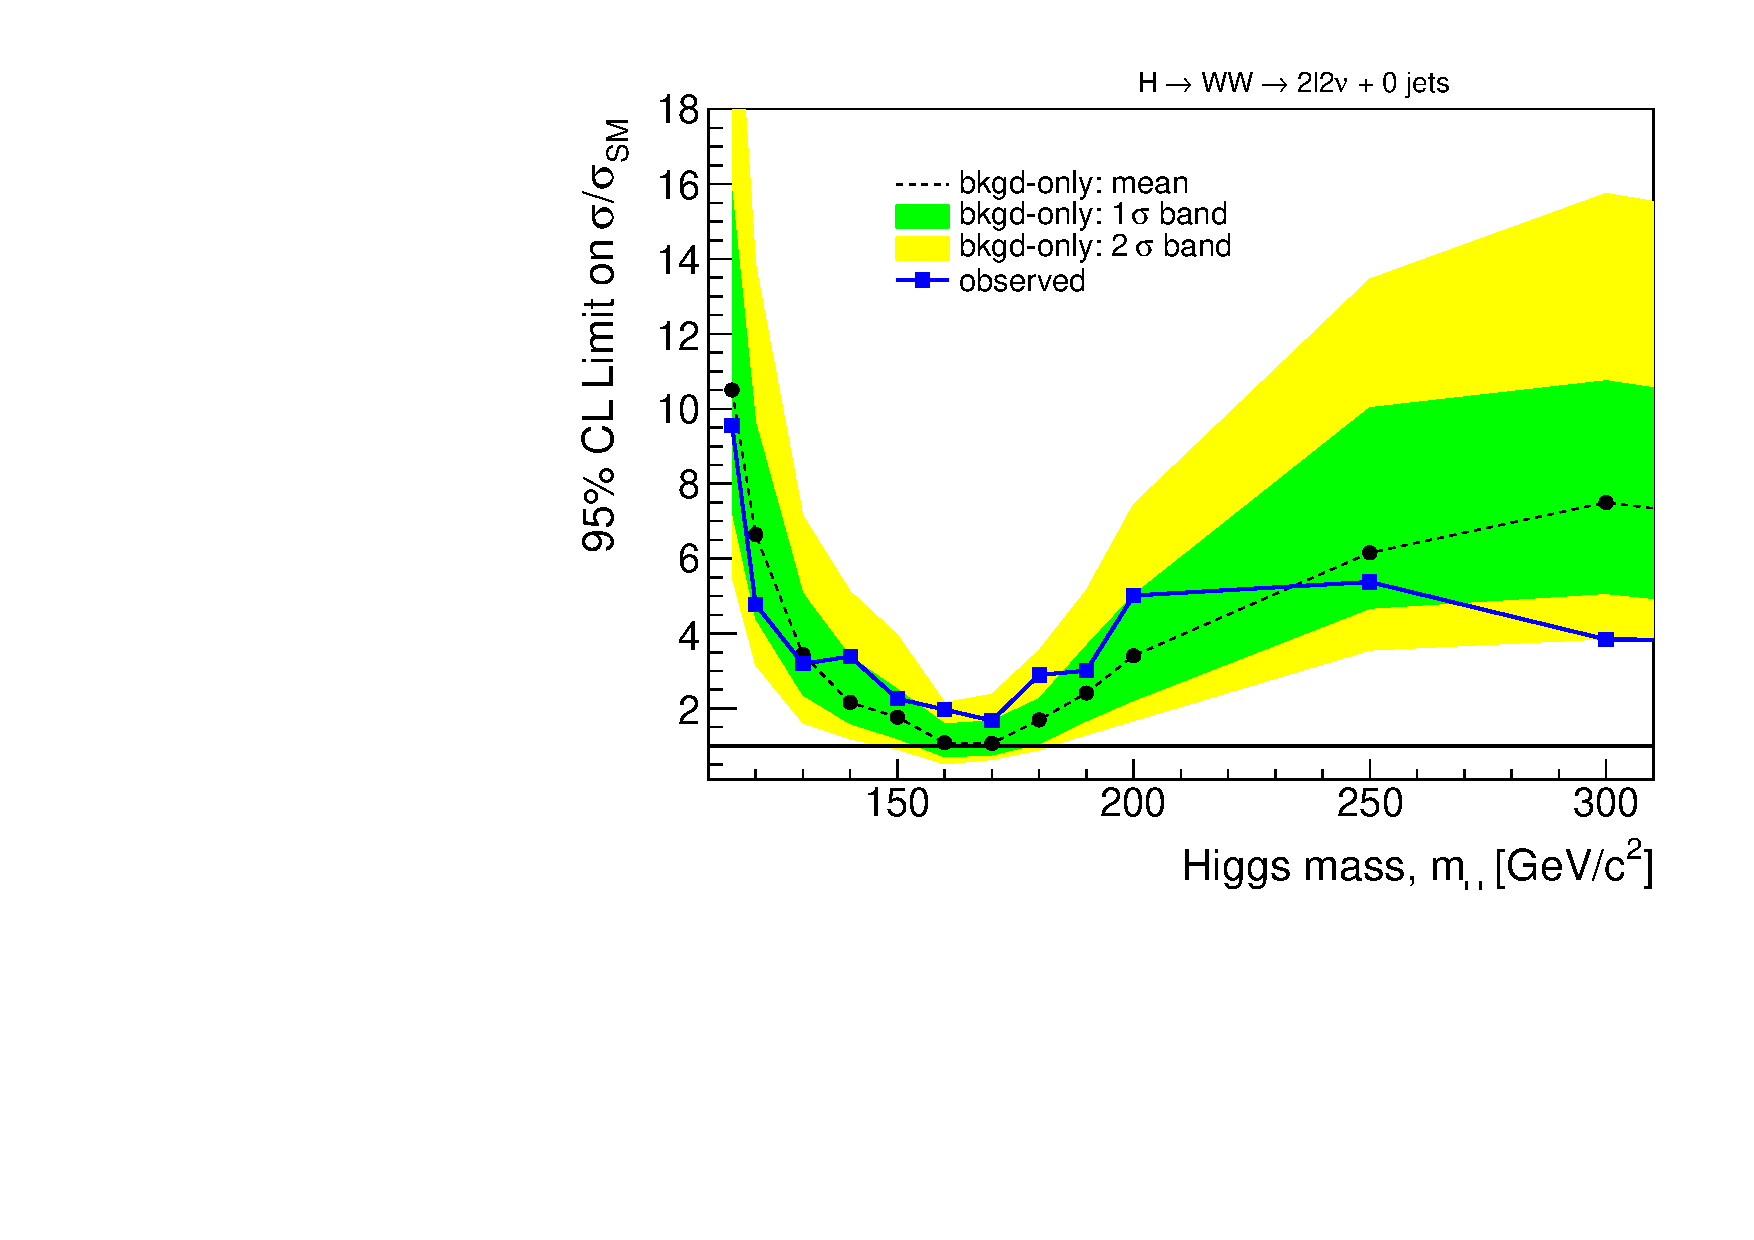
\includegraphics[width=0.49\textwidth]{figures/limits_0j_200pb_mva_1.pdf}
%%    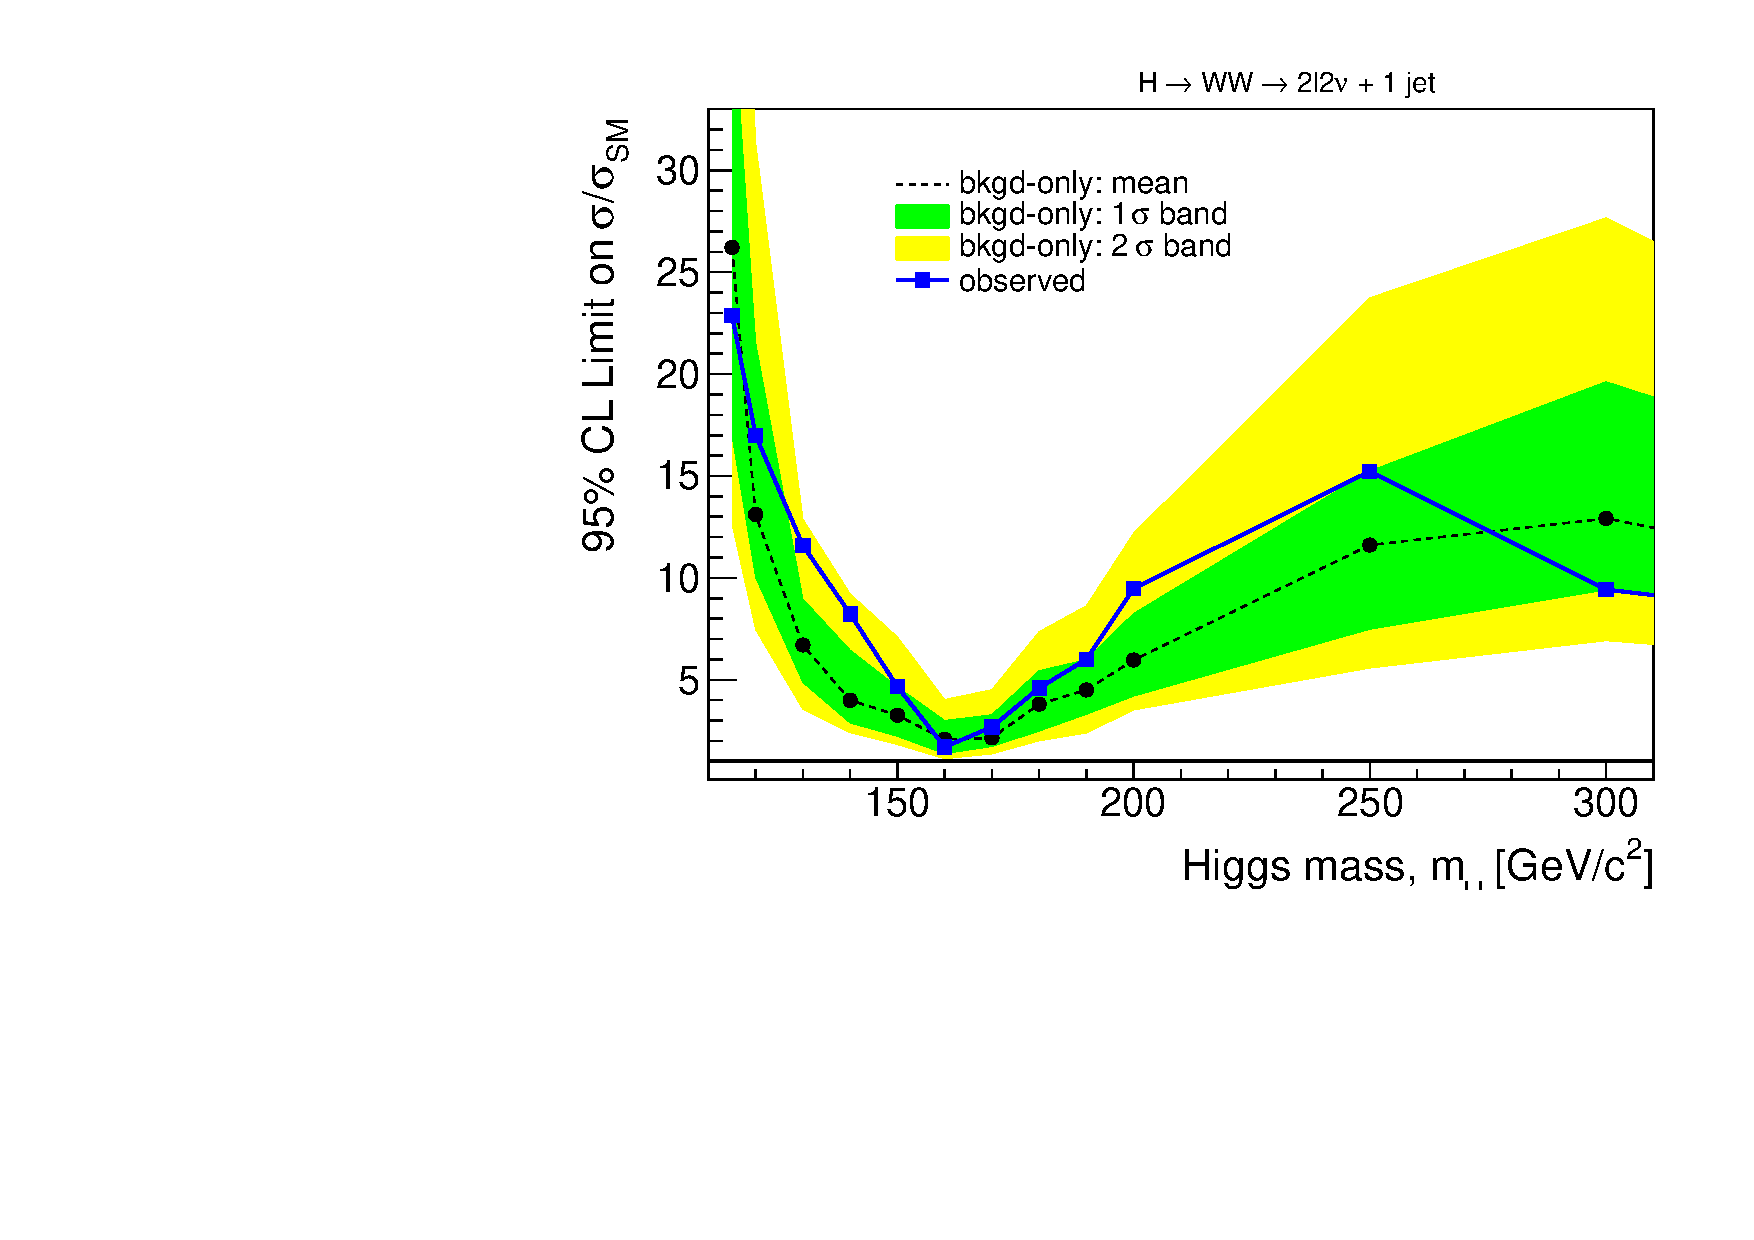
\includegraphics[width=0.49\textwidth]{figures/limits_1j_200pb_mva_1.pdf}
%%    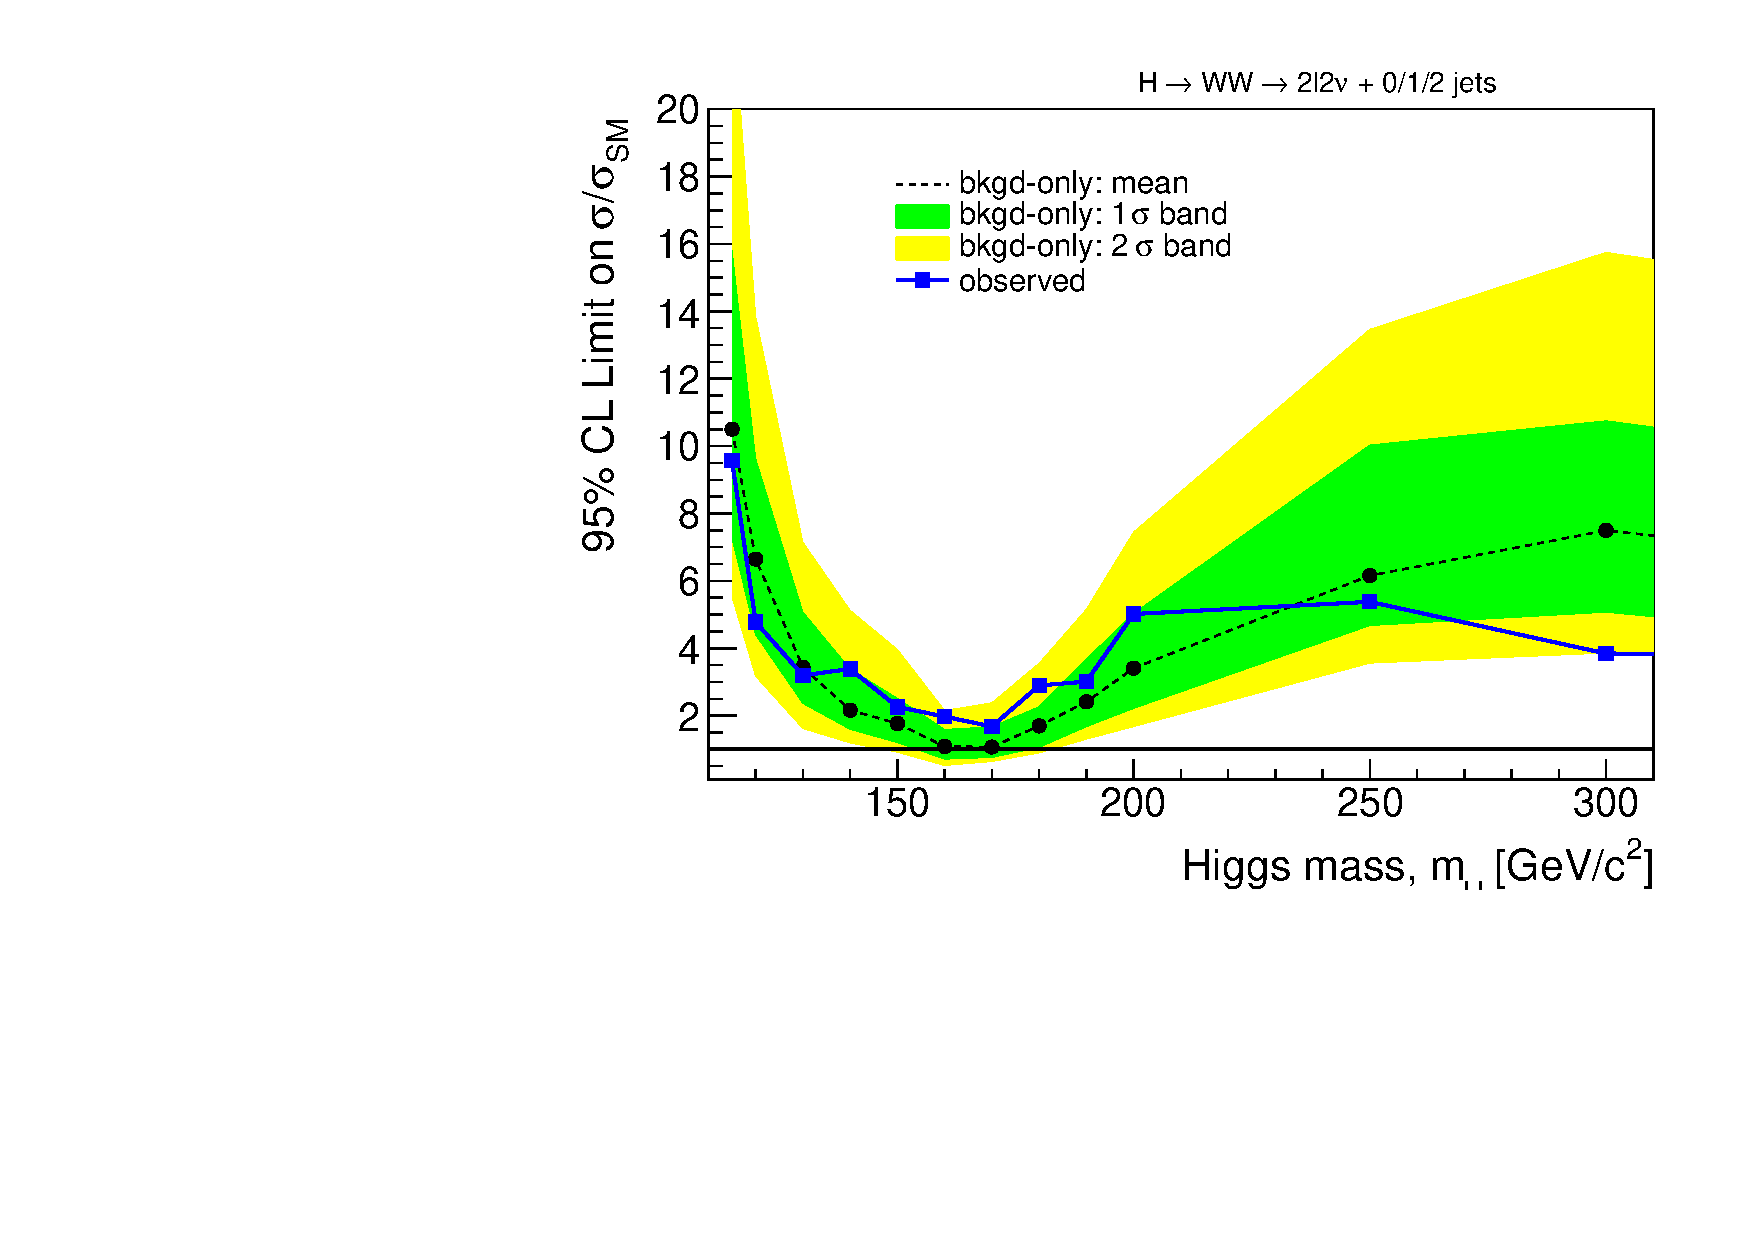
\includegraphics[width=0.49\textwidth]{figures/limits_nj_200pb_mva_1.pdf}
%%    \caption{Multivariate analysis upper limits at 95\% C.L. for \intlumi of data. Top left plot 
%%    is the result for the 0-jet bin, top right plot is the result for the 1-jet bin and, 
%%    bottom right plot is the combined result.}
%%    \label{fig:mvabase_uls_data}
%% \end{center}
%% \end{figure}

\cleardoublepage
